\chapter{Articulações intra-partidárias e as eleições para prefeito no Brasil}
\label{cap:eleicoes}

Em fevereiro de 2010 o jornal o Estado de Minas publicou uma notícia na qual relatava que Marcus Pestana (PSDB-MG), até o início daquele ano secretário de Estado da Saúde de Minas Gerais, causou mal-estar na Assembléia Legislativa do estado. O ex-secretário havia enviado ambulâncias e recursos para os serviços de saúde dos municípios com o objetivo de atrair para sua própria candidatura o apoio de prefeitos comprometidos eleitoralmente com outros deputados de seu partido ou de partido aliados. Até descobrirem que Marcus Pestana não se candidataria a deputado estuadal, mas sim a deputado federal (cargo para o qual foi eleito naquele ano), os parlamentares aliados do então governador Aécio Neves (PSDB-MG) no Legislativo estadual apresentaram queixas ao chefe do Executivo (e liderança central no PSDB do estado) de que Marcus havia ``invadido'' suas bases eleitorais. 

A notícia relatava também que Elbe Brandão (PSDB-MG), deputada estadual e então secretária de Estado Extraordinária para o Desenvolvimento dos Vales do Jequitinhonha e Mucuri e do Norte de Minas, provocava reação semelhante de seus pares na Assembléia Legislativa, sobretudo entre os deputados que tinham votos concentrados no norte de Minas Gerais. Mesmo sem se recandidatar, Elbe Brandão era acusada de usar sua posição privilegiada no governo do estado para atrair prefeitos para a candidatura de seu marido ao Legislativo estadual.

Esses dois exemplos, dentre vários outros que se pode coletar no anedotário político, ressaltam um aspecto fundamental presente nas eleições nacionais e estaduais: a importância do apoio eleitoral de prefeitos. A notícia nos leva a crer que os prefeitos são eleitoralmente importantes a ponto de membros do mesmo partido disputarem seu apoio e recorrerem à hierarqui partidária para resolver o conflito de quem receberá o apoio dos líderes municipais. É possível encontrar diversos outros relatos sobre candidatos a cargos majoritários que também competem por prefeitos em suas campanhas. Esta disputa, porém, acontece normalmente fora das instâncias do partido. %\footnote{
%http://www1.folha.uol.com.br/poder/755480-prefeitos-do-pr-mg-se-rebelam-e-fazem-manifesto-por-anastasia.shtml
%http://www1.folha.uol.com.br/poder/769990-helio-costa-acusa-psdb-de-aliciar-prefeitos-em-minas.shtml
%http://www1.folha.uol.com.br/multimidia/podcasts/792407-tucanos-temem-migracao-de-apoio-dos-prefeitos-nos-estados-ouca-analise.shtml
%http://www1.folha.uol.com.br/poder/837880-pps-expulsa-prefeito-que-apoiou-dilma-e-ameaca-infieis-da-sigla.shtml
%http://politicaemdia.wordpress.com/2010/02/17/deputados-disputam-prefeitos-no-periodo-pre-eleitoral/} 

O ponto de partida da tese é justamente examinar se prefeitos são capazes de mobilizar apoio eleitoral para seu próprio partido durante seu mandato. Olhando para este problema por outro ângulo podemos reescrever a pergunta: os partidos são capazes de produzir articulações partidárias entre políticos de diferentes níveis de governo?

Articulação partidária é um problema bastante crítico em um sistema político como o brasileiro. Em primeiro lugar, a existência de múltiplos partidos complexifica e amplia as possibilidades de alianças. Coligações eleitorais e coalizões de governo são parte do cotidiano da política partidária no Brasil, mesmo que não necessariamente acordos entre políticos requeiram alianças formais.

Em segundo, o próprio arranjo federativo contribui para dificultar a coordenação dentro das organizãções partidárias, uma vez que as disputas entre partidos não se repetem necessariamente entre estados ou nacionalmente. O caráter federativo do sistema político é, em alguma medida, também um aspecto marcante das organizações partidárias no Brasil. É comum, por exemplo, diretórios municipais se rebelarem, ou ameaçarem se rebelar, contra as decisões estuduais do partido ou diretórios estudais descumprirem determinações estabelecidas pelas lideranças nacionais.

Por fim, a adoção de lista aberta em eleições proporcionais para os cargos do Legislativo torna a eleição de parlamentares um empreendimento que necessariamente tem um componente pessoal. A competição entre candidatos de um mesmo partido, que em outros países ocorre dentro da própria organização para determinar o ordenamento na lista do partido, é transferida para a eleição. Segundo se convencionou na literatura acadêmica e no debate político, as regras eleitorais dão origem ao \emph{voto pessoal} no Brasil, cujos efeitos perniciosos são sentidos em diversas instâncias do sistema político \citep*{Ames1995,Ames1995a,Ames2001,Carey1995,Mainwaring1991,Mainwaring1999}. O \emph{voto pessoal} seria mais um aspecto sistêmico a tornar a tarefa de coordenação dentro do partido mais árdua. 

Há que se questionar -- como se pretender neste capítulo -- se o fato de os parlamentares de um mesmo partido competirem eleitoralmente entre si, terem rivalidades políticas variantes de acordo com o território e possibilidades múltiplas de alianças dentro e fora do partido faz com que os partidos brasileiros percam por completo a capacidade de articular seus membros, de estabelecer estratégias coordenadas e, no limite, de estruturar a competição eleitoral. Neste capítulo, o exame do papel dos prefeitos nas eleições nacionais e estaduais tem como objetivo rever esta interpretação bastante disseminada nas análises sobre a política brasileira. Em um sistema onde membros de um mesmo partidos não se coordenam entre si, não deveríamos observar efeitos relevantes da vitória eleitoral em um nível de governo no desempenho do partido em outro nível.

Este problema de pesquisa não é inédito. Segundo \citet{Ames1994}, o apoio eleitoral de prefeitos é um elemento chave no sucesso de candidaturas presidenciais. Prefeitos são, de determinado ponto de vista, cabos eleitorais privilegiados e cujo apoio é crucial para o sucesso de quem busca votos no município. \citeauthor{Ames1994} denominou esse fenômeno de ``efeito \emph{coattail} reverso''. Empiricamente, \citeauthor{Ames1994} examinou a correlação entre a filiação do prefeito e o desempenho de cada candidato na eleição presidencial. Sua conclusão, a partir dos resultados da eleição de 1989, é a de que candidatos à presidência têm desempenho superior nos municípios nos quais seu partido governa.

Ainda que \citeauthor{Ames1994} seja um dos principais advogados da fragilidade dos partidos políticos brasileiros, seu trabalho produziu evidências de que as eleições municipais estão conectadas com as demais e, portanto, sua tese acaba por ressaltar este aspecto importante do sistema eleitoral brasileiro. \citet{Carneiro2008} avançaram neste problema ao demonstrar que há correlação entre a votação dos partidos para os diferentes níveis e ramos de governo, incluíndo as eleições para prefeito. Ambos trabalhos sugerem que, a despeito das regras eleitorais produzirem incentivos para dispersão, indisciplina e ausência de cooperação dentro dos partidos, há coordenação intra-partidária na arena eleitoral.

Na tentativa de avançar o debate sobre a coordenação intra-partidária, o primeiro objetivo da tese é avaliar o impacto das eleições para prefeito no desempenho do partido nas demais eleições e reexaminar a hipótese de \emph{coattail} reverso de 1996 a 2010. Mais especificamente, o objetivo é estimar o impacto da vitória nas eleições para prefeito no desempenho dos candidatos do partido a deputado federal, deputado estadual, senador, governador ou presidente\footnote{Parte dos resultados já foram publicados no artigo \citet*{Avelino2012} \emph{Articulações intrapartidárias e desempenho eleitoral no Brasil}, publicado na Revista Dados. Neste capítulo, amplio a análise apresentada no artigo para outros anos eleitorais, outros cargos e atento a possíveis efeito heterogêneos no impacto da vitória nas eleições municipais sobre o desempenho do partido nas demais eleições.}. A escolha deste horizonte de tempo é limitada pela inexistência de dados de qualidade sobre as eleições para prefeito anteriores a 1996. As eleições de 2010 são as últimas eleições nacionais e estaduais brasileiras e apenas em 2014 será possível observar os efeitos das eleições de 2012.

Há várias diferenças entre o que se empreende neste capítulo e os trabalhos que tratam do tema na literatura, a começar pela própria compreensão do fenômeno em questão. Em primeiro lugar, o efeito \emph{coattail} apareceu originalmente na como explicação para o impacto do desempenho presidencial -- medido como popularidade do presidente ou como performance macroeconômica do país -- nas chances de vitória dos membros do partido do presidente nas eleições legislativas e nos níveis subnacionais de governo. Interessa para esta pesquisa, contudo, apenas o efeito do partido governar o município no desempenho eleitoral para os demais cargos. Não importa o quão bem sucedido o prefeito é ao longo do mandato: importa se é capaz de mobilizar votos para seu próprio partido estando à frente da prefeitura.

Dessa forma, não há interesse na correlação entre a performance do partido nas eleições municipais e nas demais eleições. A correlação entre eleições pode ser sintoma de diversos outros fenômenos. Pode, por exemplo, significar a consolidação da imagem dos partidos perante o eleitorado e a consequente redução da volatilidade eleitoral. Ou ainda, pode ser resultado do efeito \emph{coattail} que presidentes ou governadores provocam sobre as candidaturas de seu partido -- e não necessariamnete do efeito \emph{coattail} reverso. O impacto da vitória no município nas demais eleições é um dos muitos possíveis fenômenos capturados pela semelhança entre a performance do partido em diferentes eleições no mesmo município.

O problema metodológico central é justamente separar analiticamente a correlação do desempenho entre eleições dos efeitos da vitória no município nas eleições subsequentes. A expectativa é que um partido tenha bons resultados nas eleições nacionais e estaduais nos municípios nos quais é vitorioso nas eleições para prefeito. A probabilidade do partido governar o município está associada aos mesmos fatores -- observáveis ou não observáveis -- que produzem boa performance nas disputas para os cargos do legislativos, para governador ou presidente. Comparar diretamente o desempenho eleitoral para qualquer cargo entre municípios em que o partido governa e municípios nos quais não governa produziria estimativas viesadas do impacto da vitória para prefeitura.

A principal diferença com relação aos trabalhos anteriores sobre o tema consiste, portanto, na estratégia analítica. Em lugar de calcular correlações, seja entre voto na sequência de eleições (como \citealp{Carneiro2008}), seja entre o partido governo municipal e o voto para os demais cargos (como \citealp{Ames1994}), utilizo um desenho de regressão descontínua (RDD) para tentar dissociar o efeito da vitória para o governo municipal nos resultados das eleições subsequentes de quaisquer outros fatores, observáveis ou não. Dadas as diferenças em relação às pesquisas anteriores, evitarei usar o conceito de \citet{Ames1994}, \emph{coattail} reverso, e trabalharei com a noção de impacto ou efeito causal da vitória no município sobre um conjunto de variáveis, inclusive o desempenho eleitoral futuro do partido. A busca da identificação correta dos efeitos causais da vitória eleitoral e sua correta estimação é um dos fios condutores da tese e a estratégia de análise utilizada neste capítulo se repete nos demais, como se verá adiante.

De forma bastante sintética, em vez de comparar todos os municípios, opto por comparar o desempenho do partido nas eleições nacionais e estaduais apenas entre municípios nos quais o partido venceu a disputa para prefeito por uma margem estreita de votos e municípios nos quais perdeu as eleições também por uma margem estreita. Evita-se, dessa forma, comparar os municípios em que um partido tem continuamente bom ou mau desempenho em eleições consecutivas e nos quais a vitória para prefeito e o bom desempenho para as demais eleições têm origem em uma terceira variável, não podendo estabelecer entre elas relação de causa e efeito. Ao comparar ``quase-perdedores'' com ``quase-ganhadores'', por outro lado, é possível obter estimativas não viesadas do efeito da vitória nas eleições municipais, pois a única diferença relevante entre eles é o fato de terem ou não sido eleitos. Desenhos de regressão descontínua têm sido amplamente utilizados na ciência política e na economia para solucionar exatamente o tipo de problema proposto nesta pesquisa. Ainda neste capítulo explico em mais detalhes o desenho de pesquisa e procedimentos adotados.

\section{Partidos políticos brasileiros na literatura: uma breve revisão do debate e o reaxame da tese distributivista}

A relevância dos partidos políticos é certamente um dos temas mais disputados na ciência política no Brasil. O debate sobre partidos brasileiros foi fortemente influenciado pelos modelos teóricos desenvolvidos para explicar o Congresso norte-americano (para o debate nos EUA ver \citealp{Cox1993}), que, em alguma medida, foram acomodados na literatura brasileira (para um balanço da literatura ver \citealp[Capítulo 1]{Carvalho2003}). Em particular, a perspectiva distributivista -- na qual os parlamentares são ponto focal da análise e cuja preocupação central são os efeitos das regras eleitorais na atuação legislativa -- teve bastante aderência nas explicações sobre o funcionamento do Congresso Nacional e, por extensão, sobre o funcionamento sistema político brasileiro como um todo \citep*{Ames1995, Ames1995a, Ames2001, Ames2011, Mainwaring1991, Mainwaring1999, Samuels1997, Carvalho2003, Pereira2001, Pereira2007, Lemos2011}. Nesta seção, discuto brevemente alguns aspectos dessa perspectiva teórica, examino alguns de seus pressupostos e busco contrastá-la com a proposta do capítulo. 

No modelo distributivista, a unidade de análise não é o partido político, mas sim o legislador individual. A autonomia do parlamentar em relação ao partido tem estatuto variante: ora é um pressuposto analítico, assumido em conjunto com a irrelevância normativa dos partidos políticos, ora é uma consequência analítica, derivada das características da competição eleitoral.

As primeiras análises sobre o Congresso Nacional brasileiro após a transição para a democracia continham elementos presentes no arcabouço analítico distributivista. Fundamentalmente, tais trabalhos pressupoem que o comportamento dos legisladores durante o mandato será condicionado pelos incentivos criados pelo sistema eleitoral. Dito de outra maneira, o resultado da arena legislativa está conectado -- ou melhor, funcionalmente subordinado -- às restrições enfrentadas pelos parlamentares na arena eleitoral. A expectativa de tais análises, portanto, é de que a forma do sistema eleitoral -- a fórmula de conversão de votos em assentos e o tamanho e a magnitude dos distritos -- contribua para moldar o desenho institucional da casa legislativa e influencie o tipo de produção parlamentar, normalmente identificada entre produções mais universais ou mais particularistas, ou seja, geograficamente concentrada e/ou focada em grupos políticos e sociais específicos. 

Uma parte considerável da produção sobre o Congresso Nacional brasileiro adotou a perspectiva distributivista. Ames, um dos mais proeminentes autores desta vertente, relaciona diretamente os problemas de governabilidade à adoção do sistema proporcional com lista aberta para as eleições legislativas (\citealp{Ames2001}). A fórmula eleitoral adotada no Brasil, segundo tal perspectiva, reduziria o controle que os partidos têm sobre seus candidatos na eleição e, consequentemente, enfraqueceria o controle sobre os parlamentares de suas bancadas.

Sob a ótica distributivista, os candidatos de um partido têm um incentivo claro:  ``cultivar o voto pessoal'' \citep*{Ames1995, Ames1995a, Ames2001, Carey1995, Mainwaring1991, Mainwaring1999}. As estratégias de campanha não são partidárias, mas sim estritamente individuais, sendo esta uma das características mais distintivas de nosso sistema eleitoral. Os incentivos perversos presentes no sistema político brasileiro -- segundo a literatura distributivista -- são cumulativos: para sedimentar sua imagem pessoal no eleitorado e obter votos para se reelegerem, os parlamentares direcionam seus esforços no Congresso Nacional para a obtenção de benefícios desagregados para suas bases eleitorais e utilizam expedientes como a patronagem e o clientelismo para perpetuar sua popularidade no eleitorado. Os partidos políticos seriam secundários na construção de carreiras políticas nacionais.

Uma das consequências de partidos da irrelevância dos partidos é que os vínculos entre políticos de diferentes níveis de governo na federação não importam. Políticos de diferentes partidos podem formar alianças de acordo com a conveniência da conjuntura eleitoral. De fato, exagerando esta perspectiva, chegaríamos a um ponto em que as alianças políticas em eleições seriam desencessárias. Não haveria razões para a exitência de vínculos partidários entre prefeitos e deputados federais, por exemplo, uma vez que o funcionamento eleitoral se assemelharia ao de um mercado no qual as transações dentro e fora dos partidos têm o mesmo custo. No limite, a construção de organizações partidárias complexas, que conectem membros locais do partido às lideranças nacionais não importa, uma vez o fator determinante para um carreira política de sucesso é a sedimentação da imagem pessoal junto a um grupo de eleitores geograficamente concentrados e para o qual os eforços ao longo do mandato são direcionados.

Na ausência de distritos bem delimitados como no sistema eleitoral norte-americano, obter benefícios desagregados para suas bases eleitorais é normalmente traduzido, para o caso brasileiro, como concentrar geograficamente o envio de recursos orçamentários para os municípios onde o parlamentar obteve mais votos nas eleições anteriores\footnote{Este é um tema explorado com mais cuidado no Capítulo~\ref{cap:emendas}.}.

A irrelevância dupla dos partidos políticos, como elemento da análise e como consequência da análise, é, portanto, um aspecto marcante das análises distributivistas. A primeira pergunta que um analista deve fazer, no entanto, é: será que a ausência de evidências de cooperação interna nos partidos políticos não é resultado da própia construção da análise focado no individualismo parlamentar? Ou ainda, será que a existência de incentivos para a atuação individual dos parlamentares implica necessariamente na anulação do papel dos partidos políticos como estruturas que organizam a competição eleitoral, promovem coordenação entre políticos do mesmo partido e conectam lideranças em diferentes níveis de governo? Este capítulo contribui para a literatura testando se há evidências de coordenação intra-partidária no Brasil.

Alguns exageros da perspectiva distributivista já foram mitigados, nos EUA e no Brasil, pelos trabalhos que investigaram a atuação dos partidos políticos no Congresso Nacional. \citet{Cox1993} realizaram um dos esforços teóricos e empíricos mais notórios para se analisar a atuação dos partidos dentro das casas legislativas e deram origem ao que se denominou \emph{modelo partidário}. Se a influência das inovações teóricas que surgiram na análise do Legislativo norte-americano na literatura brasileira não foi direta, os trabalhos produzidos no Brasil guardam bastante semelhança com essa literatura, sobretudo, em suas implicações analíticas: a existência de efeitos dispersivos do sistema eleitoral não necessariamente se tornam efetivos no Legislativo.

No Brasil, os estudos sobre o comportamento dos partidos no Congresso produziram da metade da década de 90 em diante uma guinada analítica \citep{AmorimNeto2001, AmorimNeto2003, Figueiredo1999a, Figueiredo2000, Figueiredo2002, Figueiredo2008, Limongi2005, Santos1997, Santos1999, Santos2002}. As análises distributivistas foram confrontadas por trabalhos preocupados em examinar de forma mais detalhada o comportamento dos parlamentares brasileiros no Congresso Nacional. \citeauthor{Figueiredo1999a} foram os primeiros a apontar, contrariando os prognósticos negativos sobre o impacto das regras eleitorais na atuação legislativa, que os parlamentares brasileiros votam disciplinadamente na Câmara dos Deputados, seguindo as indicações de seus respectivos líderes partidários \citep{Figueiredo1999a}. Os partidos, e não os legisladores individuais, estruturam as relações do Legislativo com o Executivo e  organizam o processo decisório no Congresso Nacional.

No caso brasileiro, a distribuição de poder dentro da Câmara dos Deputados -- que concentra poder na mesa diretora e nas lideranças -- e as regras de elaboração e execução do orçamento federal dificultam o acesso dos parlamentares individuais às decisões que produziriam políticas distributivistas. \citeauthor{Figueiredo1999a} apontam como a estrutura do processo decisório do orçamento federal restringem o espaço de expressão dos interesses individuais dos parlamentares \citep{Figueiredo1999a,Figueiredo2008}.

Os incentivos para a atuação individualista dos parlamentares brasileiros, portanto, não caracterizam a atuação coletiva do Congresso Nacional. Em outras palavras, as regras eleitorais não necessariamente afetam os partidos no Legislativo \citep{Desposato2008} Mesmo sob o efeito de incentivos para a dispersão e particularização da atividade parlamentar, os partidos são a chave analítica para a compreensão do Legislativo nacional. Inclusive o processo de elaboração de emendas individuais ao orçamento, que deveria refletir os interesses particularistas dos parlamentares, opera dentro de parâmetros estabelecidos pelos partidos. Se há evidências de que a atividade legislativa está estruturada em torno dos partidos políticos, por que esses mesmos partidos não seriam elementos fundamentais para a compreensão da competição eleitoral? Podem os partidos políticos serem, ao mesmo tempo, os elementos centrais da atuação legislativa e inoperantes nas eleições?

\citeauthor{Pereira2003} defendem que não há contradição na existência de partidos fracos na arena eleitoral e partidos fortes no Congresso \citep{Pereira2002,Pereira2003}. Mesmo que as lideranças sejam mediadoras nas negociações para execução de emendas com o Governo Federal em troca de votos no Congresso, os deputados continuam a ter influência sobre o destino de tais recursos. Seguem as indicações das lideranças partidárias no Congresso Nacional estrategicamente para obter em troca os recursos necessários para sua sobrevivência eleitoral, ou  o que se denominou na literatura americana de ``pork barrel''. Sob esta ótica, a inconsistência central do modelo distributivista estaria na desconsideração das regras internas ao Congresso Nacional e não na avaliação negativa sobre os partidos no eleitorado e sobre a atuação autônoma dos candidatos.

Cabe, então, examinar com mais cuidado alguns dos pressupostos da literatura distributivista sobre o funcionamento da arena eleitoral.

\subsection{Revendo alguns dos pressupostos distributivistas na arena eleitoral}

A perspectiva distributivista, ao focalizar as estratégias eleitorais dos parlamentares, parte de pelo menos um dos seguintes pressupostos sobre a relação entre representantes e representados, ambos ainda pouco examinados empiricamente. O primeiro é que o político ou candidato é capaz de obter votos ao reclamar crédito pelos benefícios que obteve para a localidade ao longo de seu mandato. Segundo \citet*{Ames2011}, os eleitores são ``famintos por \emph{pork}'' e a existência de demanda garante que os investimentos em políticas distributivistas trarão resultado eleitoral.

Trata-se, porém, de um pressuposto demasiadamente forte. De um lado, é preciso acreditar que o parlamentar consiga reclamar crédito pelo benefício concedido a um grande número de eleitores e ainda que estes eleitores se lembrem de sua atuação em benefício da localidade. Em um contexto no qual os eleitores têm pouca memória sobre os seus próprios votos em eleições anteriores, manter viva para o eleitor a lembrança de uma atuação legislativa em prol da localidade é uma tarefa bastante árdua. O risco para os deputados que buscam reeleição é demasiadamente alto para confiar apenas na sedimentação de sua imagem individual perante o eleitor -- seja como efeito inercial da última eleição ou como resultado do fortalecimento de sua imagem durante o mandato.

Ademais, pela própria lógica da construção do orçamento, os  benefícios localizados podem assumir, em geral, duas formas: a execução de políticas federais ou estaduais na localidade, ou, mais provavelmente, a transferência de recursos mediante convênios, seja para prefeituras ou para entidades sem fins lucrativos. Como apontam \citeauthor{Pereira2003}, mesmo que os partidos políticos restrinjam a ação individual dos deputados federais, continua havendo espaço para que os parlamentares insiram no orçamento emendas individuais que beneficiem suas localidades e que posteriormente podem sexecutadas pelo Governo Federal\citep{Pereira2003}. Estes recursos, porém, não podem jamais ser direcionados diretamente ao eleitor e a relação entre emendas, voto e reeleição não é clara \citep{Mesquita2008}. O Capítulo~\ref{cap:emendas} trata do assunto em mais detalhes.

O segundo pressuposto por vezes adotado na perspectiva distributivista, em contraste, é bastante mais plausível do que assumir os demandantes de benefícios particularistas como sendo os eleitores de determinadas localidades. Os recursos obtidos por um parlamentar não são enviados aos eleitores, mas a apoiadores políticos capazes de mobilizar votantes durante as eleições. Castro et al. listam alguns desses apoiadores centrais: prefeitos, vereadores, empresários, líderes comunitários ou sindicais, religiosos, professores e comunicadores de massa, qsuase todos no rol de potenciais dirigentes de organizações legalmente habilitadas a se beneficiar de transferências de recursos dos governos federal e estaduais \citep{Castro2009}). Não são, portanto, os eleitores os receptores diretos dos benefícios obtidos pelos parlamentares. Do ``lado da demanda'' estão lideranças locais, que podem ou não transformar tais recursos em políticas que atinjam o cidadão e proporcionem retorno eleitoral.

Por fim, há quem argumente ou assuma implicitamente que essas localidades são de fato os municípios \citep{Carvalho2003, Pereira2001, Pereira2007}. Na análise da relação entre deputados e suas bases eleitorais, em lugar de adotar a definição cartográfica ou administrativa, podemos definir localidade utilizando um critério político: a existência de apoiadores políticos que sistematicamente são capazes de influenciar o voto de eleitores. Ainda assim, considerando que os prefeitos e vereadores são alguns dos mais importantes ``cabos eleitorais'' nas eleições legislativas, podemos igualar as definições política e administrativa, sendo que o município pode ser adotado como unidade territorial para fins analíticos.

Nesta tese, parte-se do pressuposto de que não existem eleitores geograficamente concentrados que demandam benefícios aos parlamentares, mas sim atores políticos de influência geográfica limitada que estão dispostos a mobilizar votos para os candidatos em troca de benefícios às organizações das quais fazem parte. Os prefeitos, espera-se, são os atores mais relevantes desse conjunto, seja pelos recursos dos quais dispõem (possibilidade de contratar e demitir servidores, executar políticas, etc), seja pela posição de político bem votado no município, ou ainda pelo fato de que a maior parte das transferências federais e estaduais para localidades que podem ser inseridas no orçamento por parlamentares assume a forma de transferências a prefeituras.

A capacidade dos prefeitos afetarem postivamente as campanhas nas quais se engajam é uma questão sujeita a vefiricação empírica. O teste do potencial dos prefeitos como cabos eleitorais está embutido no exame do efeito da vitória do partido nas eleições municipais sobre a performance do partido nas demais eleições. Como foi apontado na introdução deste capítulo, para estimar tal efeito, é necessário adotar estratégias metodológicas que permitam separá-lo dos fatores que explicam o desempenho eleitoral do partido ao longo de diferentes eleições. Na próxima seção apresento os procedimentos de pesquisa deste capítulo, que são semelhantes aos procedimentos adotados nos Capítulos~\ref{cap:emendas} e~\ref{cap:mecanismos} da tese, e descrevo com detalhes o uso de desenhos de regressão descontínua para estimar o efeito da vitória nas eleições municipais no Brasil em uma determinada variável de interesse.

\section{Procedimentos de Pesquisa: Regressão Descontínua e as eleições para prefeito no Brasil}

Desenhos de regressão descontínua (RDD) se tornaram bastante comuns na ciência política desde a publicação do artigo de Lee em 2008 sobre as vantagens do incumbente nas eleições legislativas nos EUA \citep{Lee2008}. O uso deste tipo específico de desenho de pesquisa faz parte do ressurgimento do interesse por estratégias analíticas que permitam a identificação de efeitos causais, que caracterizou sobretudo a literatura sobre avaliação de políticas e programas na economia (para balanços da literatura, demonstrações e críticas ver \citealp*{VanderKlaauw2008, Angrist2008, Lee2008, Imbens2008, Imbens2009, Lee2010a, Dunning2012, Eggers2013}). Essencialmente, desenhos de regressão descontínua aproveitam a existência de um mecanismo de atribuição de ``tratamento'' (ou condição) a unidades (ou indivíduos) que ultrapassam determinada ``fronteira'' em um determinado atributo, em geral representado por uma variável contínua. Alguns exemplos de descontinuidades são a inclusão de beneficiários em uma política pública a partir de um determinado nível de renda/idade/escolaridade, a aprovação em um programa de treinamento ou curso para indivíduos que obtêm uma nota acima de um ``corte'', o tratamento diferenciado nas regras fiscais/eleitorais a municípios a diferentes faixas de população. Na Brasil há diversos trabalhos recentes que utilizam RDD em ciência política (ver \citealp*[pp. 70]{Dunning2012} para uma lista de trabalhos no Brasil e em outros países; no Brasil, alguns dos trabalhos que utilizam RDD para estimar efeitos causais são: \citealp*{Ferraz2008, Litschig2009, Caughey2011, Boas2011, Fujiwara2011, Titiunik2011, Avelino2012, Brambor2012, Brollo2012, Brollo2013}).

Em situações como esta, unidades que quase ultrapassaram a fronteira (ou seja, não ultrapassam) são bastante semelhantes em características observáveis e não observáveis a unidades que ultrapassaram a fronteira por muito pouco e às quais, portanto, o tratamento é atribuído. Se o tratamento tem efeito em alguma variável de interesse, a comparação entre unidades imediatamente abaixo e imediatamente acima da fronteira deve revelar o efeito causal do tratamento sobre tal variável.

Desenhos de regressões descontínuas são particularmente interessantes para a ciência política, pois eleições majoritárias produzem descontinuidades que podem ser exploradas para estimar o efeito da vitória -- ou, alternativamente, do partido que venceu as eleições governar -- sobre um conjunto diversos de variáveis (exemplos da aplicação de RDDs em eleições podem ser encontrado em \citealp*{Lee2008, Pettersson-Lidbom2008, Boas2011, Titiunik2011, Avelino2012, Brambor2012, Brollo2012, Fowler2012, Pettersson-Lidbom2008}). Eleições majortiárias determinam o resultado da eleição por um mecanismo fixo: ter o maior número de votos dentre todos os candidatos. Em uma eleição com apenas dois partidos, aquele que obtém mais da metade dos votos -- descontados abstenções, nulos e brancos -- está eleito. Em uma eleição com três ou mais candidatos, o partido com margem de vitória positiva em relação a todos os demais vence a disputa.

Nesta seção, examino com cuidado os fundamentos desse tipo de desenho de pesquisa aplicado a eleições. A seguir, apresento os dados utilizados no capítulo. Ao final da seção, realizo alguns testes para verificar a validade do RDD utilizado neste capítulo.

\subsection{Regressão Descontínua e as eleições para prefeito no Brasil}

A votação de um partido $p$ no município $m$ em uma eleição para prefeito no ano $t$  ($V_{p,m,t}$ ou $V_{i}$, sendo $i$ uma combinação de $p$, $m$ e $t$) pode ser descrita em termos de uma função densidade de probabilidade condicional às diversas características do partido no município -- tais como número de apoiadores, qualidade do candidato, aspectos da campanha, imagem perante o eleitorado, etc -- e por um termo aleatório $\epsilon_{i}$. Esses fatores que descrevem $V_{i}$ são representados por $A_{i}$ e parte deles raramente é observável ao pesquisador. Para simplificar a descrição da mecânica do RDD, vou assumir que nenhum dos componentes de $A_{i}$ é observável. 

No Brasil, em municípios com menos de 200 mil eleitores aptos, os candidatos disputam uma eleição majoritária de apenas um turno para a prefeitura. O tratamento -- vencer as eleições para prefeito -- também obedece a um mecanismo fixo: vence as eleições o candidato que obtiver o maior número de votos $V_{i}$ (independentemente de ter atingido ou não a metade mais um dos votos válidos). Em outras palavras, o partido vitorioso ($d_{i}=1$) é aquele que tiver margem de votos positiva em relação ao partido oponente mais bem votado ($\tau_{i}>0$; o símbolo $\tau$ representa a letra grega ``tau'') e terminar a eleição em primeiro colocado. Partidos com margens de votos negativas ($\tau_{i}<0$) em relação ao partido mais bem votado não são eleitos ($d_{i}=0$).  Neste caso, o tratamento $d_{i}$ é função de $\tau_{i}$ e, portanto, não é independente dos fatores representados por $A_{i}$. Espera-se, assim, que cada partido tenha uma probabilidade diferente de ser ou não eleito (tratado) dado $A_{i}$.

Uma variável de resultado ($Y_{i}$) qualquer pode ser descrita da mesma maneira, ou seja, como função dos fatores presentes em $A_{i}$, dos quais a votação do partido nas eleições para prefeito também depende, e também de $V_{i}$, que são os votos recebidos na eleição para prefeito. O voto para deputado federal nas eleições seguintes, o total de recursos enviados via emendas ao município pelos deputados federais do partido ou o total de recursos arrecadados para as campanhas futuras no município -- variáveis de interesse nesta tese -- são exemplos da variável de resultado $Y_{i}$.

Como $\tau_{i}$ e $Y_{i}$ são funções da mesmo conjunto de fatores não observáveis e $d_{i}$ é função de $\tau_{i}$, não é possível afirmar que $Y_{i} \perp d_{i}$, ou seja, que o tratamento independe da variável resposta. A condição de independência neste caso é $Y_{i} \perp d_{i} | A_{i}$, novamente, sendo que há componentes de $A_{i}$ que não são observáveis. Na linguagem do problema que se pretende investigar nesta tese, o desempenho do partido nas eleições para prefeito está correlacionado com o tratamento (vencer ou não as eleiões no município) e com a variável resposta -- como o voto nas eleições subsequentes para os demais cargo ou as emendas apresentadas pelos deputados do partido que beneficiem o município -- e ambas são explicadas, pelo menos em parte, por fatores que não podemos medir, como reputação, qualidade dos candidatos ou capítal político do partido no município.

Portanto, para estimar o efeito causal em $Y_{i}$ da vitória nas eleições municipais, $\rho$ (o símbolo $\rho$ representa a letra grega ``rho''), não é possível calcular apenas a diferença entre a esperança de $Y_{i}$ para os municípios em que o partido foi eleito e a esperança $Y_{i}$ onde o partido não foi eleito:\newline

\[\rho \ne E[Y_{i}|d_{i}=1] - E[Y_{i}|d_{i}=0]\]

O correto seria estimar essa diferença condicional aos fatores não-observáveis que explicam simultaneamente $Y_{i}$ e $\tau_{i}$, e, portanto $d_{i}$:

\[\rho = E[E[Y_{i}|d_{i}=1]|A_{i}] - E[E[Y_{i}|d_{i}=0]|A_{i}]\]

Contudo, $A_{i}$ são os fatores que não conseguimos medir. Tampouco é possível calcular a diferença para um partido entre os municípios nos quais perdeu e nos quais venceu controlando pela margem de votos, pois $d_{i}$ é uma função determinística da margem de votos e para cada $\tau_{i}$ há apenas tratados ou não tratados:

\[\rho \ne E[E[Y_{i}|d_{i}=1]|\tau_{i}] - E[E[Y_{i}|d_{i}=0]|\tau_{i}]\]

Ainda assim, perto da fronteira definida por $\tau_{i}=0$, unidades imediatamente acima da fronteira ($\tau_{i}=+\Delta$; o símbolo $\Delta$ representa a letra grega maíuscula ``delta'') são muito semelhantes em covariáveis às unidades imediatamente abaixo da fronteira ($\tau_{i}=-\Delta$). $\Delta$ pode ser lido como o módulo da diferença entre os dois primeiros colocados na eleição municipal, que é positiva para vencedores e negativa para perdedores. A intuição por trás desse raciocínio é que em eleições majoritárias partidos ou candidatos eleitos por uma margem muito pequena de votos são muito semelhantes (quanto à probabilidade de serem eleitos, à qualidade das candidaturas, ao apoio no eleitorado, etc) àqueles que perderam a eleição também por uma margem muito pequena de votos. Dessa forma, a probabilidade de ser eleito (tratado), $E[d_{i}]$, quando $\Delta$ tende a zero é igual para unidades logo acima e logo abaixo da fronteira que define o tratamento:

\[
\lim_{\Delta \to 0} E[d_{i}|\tau_{i}=-\Delta]=\lim_{\Delta \to 0} E[d_{i}|\tau_{i}=+\Delta]
\]

Como as unidades próximas à fronteira têm probabilidades semelhantes de serem tratadas, a comparação entre elas emula um desenho de experimento em que o tratamento é atribuído às unidades de forma aleatória, pois $d_{i}\perp\tau_{i}$ para $\tau_{i}=0$. Quanto mais próximo de zero for $\Delta$, melhor a comparação e por esta razão que RDDs fazem parte de um conjunto de estratégias analíticas e desenhos de pesquisa por vezes denominados \emph{quasi}-experimentais. No caso específico das eleições para prefeito no Brasil, ao compararmos os casos em que a eleição foi decidida por uma margem apertada de votos, estamos diante de disputas em que o partido vitorioso foi definido por fatores não controláveis pelos candidatos em disputa e, portanto, não correlacionados com a variável na qual se espera que a vitória no município tenha efeito. Assim, quando $\Delta$ for suficientemente próximo de zero a condição de independência $Y_{i} \perp d_{i}$ será válida e $\rho$ poderá ser estimado por: 

\[\rho =\lim_{\Delta \to 0} E[E[Y_{i}|d_{i}=1]|\tau_{i}=+\Delta] - \lim_{\Delta \to 0} E[E[Y_{i}|d_{i}=0]|\tau_{i}=-\Delta]\]
\[=\lim_{\Delta \to 0} E[Y_{1,i}|\tau_{i}=+\Delta] - \lim_{\Delta \to 0} E[Y_{0,i}|\tau_{i}=-\Delta]\]
\[=\lim_{\Delta \to 0} (E[Y_{1,i}|\tau_{i}=+\Delta] - E[Y_{0,i}|\tau_{i}=-\Delta])\]

Apesar de desenhos de regressão descontínua identificarem adequadamente os efeitos causais, há limites, questões não solucionadas e críticas à sua utilização. O problema central de RDDs é que nem sempre há um número de observações suficiente próximas à fronteira (que define os grupos de tratamento e controle) para estimar o efeito causal do tratamento (para um discussão sobre \emph{bandwidth choice} ver \citealp{McCrary2008, Green2009, Imbens2011}). É preciso, escolher um $\Delta$ maior que zero como critério para inclusão ou exclusão de observações na análise. Quanto maior for a margem de vitória, porém, mais longe da identificação adequada do efeito causal em um RDD.

Como definir $\Delta$ é, pois, crucial em um RDD. A literatura convencionou utilizar como $\Delta$ ideal a estimativa apresentada por Imbens e Kalyanaraman, aqui representada pelo símbolo $\Delta_{IK}$, e cuja construção depende exclusivamente da distribuição dos dados, ou seja, de $Y_{i}$ e $\tau_{i}$ \citep{Imbens2011}. Entretanto, mesmo sendo construído por um critério que não depende da arbitrariedade do pesquisador, o $\Delta_{IK}$ produz resultados não necessariamente adequados ao problema em análise. Ao construir um desenho de regressão descontínua para eleições majoritárias, parece razoável argumentar que candidatos que tiveram 15\% de diferença nos votos válidos são semelhantes entre si? Sob os critérios adotados nesta tese, não. Uma possível interpretação para analisar os efeitos da vitória eleitoral com um RDD é pressupor que a eleição foi decidida por fatores ``aleatórios''. se a diferença de votos entre primeiro e segundo colocados é pequena, até o momento em que os votos são apurados não se sabe ao certo quem é o vencedor e fatores imponderáveis podem conceder a vitória a um ou outro candidato. Uma eleição cuja diferença entre os dois candidatos mais votado é de 15\%, entretanto, tem a vitória facilmente prevista com uma pesquisa de intenção de votos e certamente não se adequada a este critério.

A solução encontrada nesta tese é não decidir por apenas uma ou algumas margens de vitória específicas, mas apresentar os resultados ($\rho$) em função de $\Delta$, marcando alguns pontos de referência ($\Delta = 10\%$, $\Delta = 5\%$, $\Delta = 2,5\%$, $\Delta = 1\%$ e $\Delta = \Delta_{IK}$) para facilitar a vizualização. Desta forma, é possível, por um lado, observar qual é o menor $\Delta$ para o qual o efeito causal é estatisticamente diferente de zero e se evita obter um resultado positivo obtido por acaso. Mais ainda, a interpretação gráfica dos resultados contribui para evitar que o resultado seja obtido por uma decisão arbitrária (na escolha de uma margem de vitória específica) ou pela utilização de uma margem inadequada ao problema (como ocorre por vezes com o \emph{optimal bandwidth estimator} de Imbens e Kalyanaraman).

A segundo aspecto questão decorrente da utilização de $\Delta>0$ é a escolha do estimador. Quando $\Delta$ é muito próximo de zero, não importa a forma funcional da densidade de probabilidade conjunta de $Y_{i}$ e $\tau_{i}$ e uma diferença de médias simples entre unidades tratadas e não tratadas corresponde ao efeito esperado do tratamento, como demonstrado acima. Entretanto, quanto maior o $\Delta$, mais importante será a definição adequada da relação entre a variável de resultado e a margem de vitória, exceto se $corr(Y_{i},\tau_{i})=0$. Como esperamos que $\tau_{i}$ e $Y_{i}$ sejam ambas funções de $A_{i}$, não podemos esperar que $corr(Y_{i},\tau_{i})=0$ sem uma análise empírica cuidadosa. Assim, além de estimar o efeito do tratamento, $\rho$, como diferença de médias, utilizo outros estimadores que levam em consideração $corr(Y_{i},\tau_{i}) \ne 0$ e incluem a margem de vitória como controle.

Três maneiras usualmente encontradas na literatura para lidar como este problema são (além da estimativa por diferença de médias): 1 - assumir que a relação entre $Y_{i}$ e $\tau_{i}$ é linear e estimar a diferença entre tratados e não tratados condicional em $\tau_{i}$ quando o limite de $\Delta$ tende a zero (\emph{local linear regression}); 2 - adotar um polinônio de ordem elevada (ou, pelo menos de terceiro grau) para descrever a relação entre $Y_{i}$ e $\tau_{i}$ e considerar todos as observações, independentemente de $\tau_{i}$, para estimar $\rho$ (\emph{global polynomial regression}); ou ainda, 3 - utilizar um polinônio de ordem elevada e estimar a diferença entre tratados e não tratados condicional em todos os graus de $\tau$ quando o limite de $\Delta$ tende a zero (\emph{local polynomial regression}). Há outros estimadores populares, como \emph{weighted kernel regression}, não utilizados nesta tese.

Assim, além de apresentar $\rho$ como diferença de médias entre grupos de tratamento e em função $\Delta$, também apresento os resultado estimando $\rho$ como diferença de médias, como uma descontinuidade em uma função linear e como descontinuidade em uma função polinomial de terceiro grau. Podemos sintetizar as três maneiras de estimar $\rho$ nas seguintes regressões\footnote{É importante notar que os modelos não contém o termo de interação entre $\tau_{i}$ e $d_{i}$. Há três razões para optar por não incluir a interação: 1 - a preferência por estimar $\rho$ da forma mais simples disponível; 2 - a expectativa de que os coeficientes de $\tau_{i}$ e do termo de intereção sejam zero quando $\Delta$ e $\tau_{i}$ tendem a zero; 3 - a obtenção de resultados preliminares que indicavam que a inclusão do termo de interção não alterava a magnitude e o sinal de $\rho$, contribuindo apenas para adicionar ``ruído'' às regressões e ampliar os intervalos de confiança. Ainda assim, repito da Anexo algumas das análise incluindo o termo de interação}:

\[Y_{i}=\beta_{0}+\rho*d_{i}+\epsilon_{i}\]
\[Y_{i}=\beta_{0}+\rho*d_{i}+\beta_{1}*\tau_{i}+\epsilon_{i}\]
\[Y_{i}=\beta_{0}+\rho*d_{i}+\beta_{1}*(\tau_{i})^1+\beta_{2}*(\tau_{i})^2+\beta_{3}*(\tau_{i})^3+\epsilon_{i}\]

Qual a razão de apresentar três formas diferentes de medir o mesmo problema? Os efeitos estimados serão mais sensíveis aos estimadores quanto maior o módulo da margem de vitória adotada ($\Delta$). Ao usar três estimadores distintos, procuro me certificar de que não foi a escolha fortuita do estimador que produziu determinado resultado. Como se verá adiante, o exame da dispersão de $Y_{i}$ próxima à fronteira de atribuição do tratamento mostrará que há razões para crer que estimar o efeito do tratamento utilizando de uma regressão linear é bastante adequado ao problema, enquanto o estimador por diferença de médias é viesado. Em diversos momentos da tese, por parcimônia, a descontinuidade em uma função linear será a única estimativa apresentada.

Por fim, se desenhos de regressão descontínua têm como virtude a validade interna dos resultados, sua principal fraqueza reside na validade externa. Os resultados estimados a partir de um conjunto de eleições cuja característica é a disputa mais acirrada para a prefeitura é válido também para as demais disputas eleitorais? Não é possível afirmar com segurança. Há, porém, duas razões para não se preocupar tanto com este problema. Em primeiro, como se verá adiante, vitórias para prefeito com grandes margens são bem mais incomuns do que eleições ``apertadas''. E, finalmente, vencer eleições municipais em que o resultado é incerto seja talvez um objetivo estratégico mais relevante para os partidos políticos do que eleger o prefeito em municípios em que a vitória é muito provável.

A seguir, apresento os dados utilizados e como cada uma das variáveis foi operacionalizada para conduzir o teste de hipóteses.

\subsection{Operacionalização da pesquisa, hipótese e dados utilizados}

Nesta tese, a unidade de análise (representada por $i$) é o partido individual ($p$) em um município ($m$) em uma determinada eleição municipal ($t$), sendo que o grupo de tratados é composto pelos partidos vencedores e o de não tratados pelos partidos que a perderam eleição. A margem de vitória, $\tau_{i}$, é simétrica para os dois primeiros colocados ($+\Delta$ e $-\Delta$), sendo negativa para o perdedor e positiva para o vencedor. Como os demais perdedores em uma eleição terão necessariamente o valor absoluto de $\tau_{i}$ maior do que os dois partidos mais bem votados e a validade do desenho de pesquisa depende da aproximação de $\tau_{i}$ a zero, apenas os dois primeiros colocados são considerados. Por exemplo, se o PDMB foi vitorioso no município de São José do Brasil (fictício) na eleição de 2008, o PSDB foi o segundo colocado e o PT terceiro colocado, apenas PDMB e PSDB farão parte da análise, sendo o primeiro no grupo de tratados ($d_{i}=1$) e o segundo no grupo de não tratados ($d_{i}=0$). O módulo da margem de vitória ($\Delta$) será a diferença de votos para prefeito entre PMDB e PSDB sob o total de votos válidos\footnote{A opção nesta tese foi calcular o percentual de votos, seja nas eleições municipais ou demais, como uma razão do total de votos válidos. Alternativamente, seria possível considerar que os eleitores que optaram por votar em branco ou nulo contribuem para a incerteza em uma eleição e poderiam influnciar o resultado final se tivessem decidido por algum candidato. Neste caso, o denominador seria o comparecimento. Entretanto, o efeito desta escolha seria produzir margens de vitória $\tau$ menores, pois o total de votos válidos é necessariamente menor ou igual ao que o número de eleitores que participaram da eleição. Ao usar votos válidos como denominador, torno a obtenção de resultados positivos mais difícil e, portanto, os resultados obtidos mais críveis.}, sendo positiva para o PMDB e negativa para o PSDB.

Da mesma maneira que foram excluídos todos os partidos que não terminaram entre os dois primeiros colocados, eleições em municípios com mais de 200 mil eleitores aptos são potencialmente problemáticas e foram excluídas. Nestes municípios, o partido que obteve $\tau_{i}$ positivo no primeiro turno não necessariamente foi o vencedor. Utilizar a votação do primeiro turno para incluir tais municípios na análise seria, portanto, um equívoco. Uma alternativa seria utilizar apenas os resultados do segundo turno, posto que somente os dois primeiros colocados interessam. Entretanto, as margens de vitória de eleições definidas em segundo turno são possivelmente diferentes das eleições em que a inexistência do segundo turno está prevista pela legislação eleitoral. Felizmente, a lista de municípios nos quais a disputa para prefeito é potencialmente decidida no segundo turno é bastante reduzida.

Esta pesquisa guarda uma diferença importante em relação a outros trabalhos sobre eleições municipais que utilizam RDDs (por exemplo \citealp*{Brollo2012, Brambor2012, Titiunik2011, Bueno2014}). Tais pesquisas adotam o município como unidade de análise e consideram como tratados os municípios em que determinado conjunto de partidos (por exemplo: partido do prefeito, partidos pertencentes à coalizão presidencial, partidos de esquerda ou mesmo apenas um partido específico) são vitoriosos, sendo os demais municípios não tratados. Na linguagem da seção anterior, $i$ é definido pelo município $m$ e na eleição $t$. A variável resposta $Y_{i}$, por esta razão também é a medida de uma característica do município (probabilidade de reeleição do prefeito, total de transferências discricionárias do governo federal, gasto público, etc) em determinado ano. Por exemplo, \citet{Brollo2012} examinam os efeitos da vitória de um partido da coalizão presidencial em um município no volume de transferências voluntárias que o governo federal repassará ao município. Assim, nas eleições de 2008, municípios em que o PT ou aliados no governo federal foram vitoriosos compõem o grupo de tratados, enquanto municípios em que outros partidos venceram integram os não tratados. Cada município em uma eleição, portanto, é incluído na análise apenas uma vez, como unidade tratada ou não, enquanto nesta tese, em regra, em cada município em uma eleição há uma unidade tratada e uma não tratada.

Uma vez que a unidade de análise adotada nesta tese é definida por partido e município em uma determinada eleição, as variáveis resposta $Y_{i}$ devem ser necessariamente medidas por partido, no município e em algum momento entre eleições municipais. Neste primeiro capítulo, a variável dependente será o desempenho do partido $p$, no município $m$ e nas eleições nacionais ou estaduais dois anos depois da eleição $t$, medido como percentual de votos válidos. No exemplo da disputa fictícia em São José do Brasil em 2008, $Y_{i}$ será medido pelo percentual de votos que PMDB e PSDB obtiveram nas eleições para deputado federal, deputado estadual, senador, governador ou presidente, calculados de forma separada para cada observação.

No Capítulo~\ref{cap:emendas}, por sua vez, $Y_{i}$ será o total de emendas transferidas para o município $m$ pelos deputados do partido $p$ nos anos seguintes a $t$. Por fim, no terceiro capítulo, $Y_{i}$ poderá ser tanto o número de filiados ao partido $p$ em $m$ nos quatro anos após $t$, as receitas de campanha do partido $p$ no município $m$ na eleição municipal seguinte a $t$ ou o tamanho da coalizão para a eleição municipal do partido $p$ no município $m$ também na próxima eleição municipal. As hipóteses que levaram à coleta e os detalhes da construção da variáveis dependentes dos demais capítulos são debatidas adiante.

A hipótese central deste primeiro capítulo é: vencer as eleições para prefeito em $t$ no município $m$ impacta diretamente no desempenho eleitoral do partido $p$ nas eleições seguintes para deputado federal, deputado estadual, senador, governador e presidente. De maneira direta, são comparadas as situações nas quais um partido $p$ qualquer venceu as eleições às situações em que este partido perdeu com a finalidade de observar se o desempenho de $p$ nas eleições nacionais é maior no primeiro caso do que no segundo. No exemplo fictício de São José do Brasil, esperamos que o PMDB tenha resultados relativamente melhores nas eleições nacionais e estaduais de 2010 neste município que em municípios onde perdeu as eleições para prefeito. Contrariamente, esperamos que o PSDB tenha resultados relativamente piores em São José do Brasil que nos municípios onde venceu a disputa para a prefeitura. Note-se que interessa mais o resultado médio para todos os partidos do que os resultados individuais.

Para que haja efeito da vitória nas eleições municipais sobre o desempenho do partido dois anos depois, duas condições devem estar presentes: 1 - os prefeitos brasileiros devem ser capazes de mobilizar votos para os candidatos que apóiam; 2 - os prefeitos do partido $p$ devem apoiar preferencialmente os candidatos do partido $p$. Uma vez que é necessário satisfazer duas condições para que a hipótese seja verdadeira, para negá-la basta que uma delas seja falsa. Dito de outra forma, a presente hipótese é construída a partir de duas hipóteses nulas: prefeitos são cabos eleitorais ineficazes; e prefeitos não apoiam preferencialmente os candidatos de seu próprio partido. É fundamental notar, portanto, que a ausência de efeito no teste empírico proposto pode signifcar que alguma dessas duas hipóteses é falsa, não necessariamenta ambas.

Da maneira com que o desempenho eleitoral nas eleições estaduais e nacionais está medido, em diversas situações $Y{i}$ será zero. Por exemplo, pode ser que o PMDB não tenha tido nenhum voto para deputado federal em São José do Brasil em 2010. Como é extremamente raro os partidos deixarem de lançar candidatos a deputado federal e estadual em algum estado -- de fato, isso acontece apenas com partidos muito pequenos -- em casos como este interpreto que o partido não obteve nenhum voto e os mantenho na análise. Contudo, este procedimento, válido para deputado federal e estadual, é equivocado para os demais cargos. Por exemplo, o PMDB não teve em 2010 candidato à presidência. O que fazer em São José do Brasil, em que o PMDB foi vencedor? Pode ser que os partidos que terminaram em primeiro ou segundo colocados em determinada eleição municipal não tenham candidatos à presidência, governo estadual e ao Senado dois anos depois. Seria equivocado utilizar na análise tais municípios atribuindo zero a $Y{i}$, pois o partido não pode ser votado nas eleições nacionais ou estaduais seguintes e $E[Y{i}] \ne 0$. O risco da inclusão de tais observações na análise é o de confundir a ausência de efeito com o fato de que os prefeitos eleitos por estes partidos provavelmente participaram ativamente da eleição, apoiando algum candidato de outro partido para senador, governador e presidente. Assim, quando se tratar de eleições para senador, presidente e governor, os partidos que não podem ser votados dois anos após a eleição municipal $t$ estão excluídos.

Uma das vantagens do desenho de pesquisa proposto é que a identificação do efeito da vitória no município em uma variável resposta que possa ser medida por partido no município e entre duas eleições municipais continua tendo validade para subconjuntos de observações. O que acontece se a capacidade de articulação dos partidos tiver aumentado ao longo do tempo? Ou se alguns partidos forem mais articulados do que outros? É possível estimar os efeitos para eleições municipais específicas, por exemplo, apenas para o ano de 2008. Ou ainda, é possível estimar os efeitos para um partido ou um conjunto determinado de partidos (maiores partidos, partidos de esquerda, partidos da coalizão federal, etc), para uma área geográfica específica do país (por região) ou conjunto de municípios (por faixa de população ou por municípios com alto grau de dependência de transferências federais e estaduais, por exemplo). A hipótese testada não se altera, apenas se delimita o conjuntos que definidos por $t$, $m$ e $p$. Assim, em diversos momentos neste capítulo exploro efeitos heterogênos da vitória nas eleições para prefeito variando tais conjuntos. O único requisito fundamental é que a probabilidade de unidades próximas à fronteira serem tratadas continue semelhante à probabilidade de não serem tratadas.

Sobre este procedimento, porém, são necessários dois alertas. O primeiro deles é que não se pode comparar estatisticamente os resultados obtidos a partir de dois subconjuntos de dados. Por exemplo, se forem produzidos resultados particulares para PMDB, PT e PSDB sobre os efeitos de vencer as eleições na perfomance do partido para deputado federal, não é possível testar estatisticamente a hipótese de que o efeito do PMDB é maior do que os efeitos de PT ou PSDB. O que se pode fazer, apenas, é apresentar os resultados dos três partidos e interpretá-los, observando eventualmente resultados maiores ou menores para um ou outro partido\footnote{Para manter a análise da maneira mais descomplicada possível, decidi não analisar efeitos heterogêneos com interações nos modelos utilizados para estimar $\rho$.}.

O segundo alerta é que, ao reduzir o número de observações, as chances de não rejeitar a hipótese nula aumentam consideravelmente. Por exemplo, se em vez de testar os resultados para o PMDB, PT e PSDB fossem observados os resultados para partidos que venceram poucas eleições municipais (por exemplo, PV e PC do B), as chances de não encontrar nenhum efeito seriam bastante grandes em virtude da ausência de observações próximas à fronteira $\tau_{i}=0$. De fato, testar a heterogeneidade por partido é uma tarefa bastante difícil uma vez que a restrição ao número de observações mina as possibilidades de um teste estatístico confiável. Os efeitos heterogêneos para outras características dos partidos, da conjuntura eleitoral ou do munípio são bastante exploradas ao longo deste capítulo.

A principal fonte dos dados da tese é o Tribunal Superior Eleitoral (TSE). De lá foram obtidos dados sobre resultados eleitorais, informação sobre os candidatos e suas contas de campanha, coligações eleitorais e filiações a partidos políticos. Parte dos dados eleitorais, entretanto, foi coletada no portal IPEADATA em vez de buscados diretamente no ``Repositório de Dados Eleitorais''. Esta escolha se deve unicamente ao fato de que há menos erros e problemas nos dados fornecidos pelo IPEA que no próprio repositório do TSE. Mesmo quando coletados no IPEADATA, a fonte primária dos dados continua sendo o TSE.

Os dados sobre emendas parlamentares ao orçamento federal provêm exclusivamente dos arquivos de emendas disponibilizados pelo Senado Federal no portal SIGA Brasil. Dados sobre população e produto interno bruto municipal provêm do Instituto Brasileiro de Geografia e Estatística (IBGE), enquanto informações sobre as Finanças Públicas municipais têm como origem a Secretaria do Tesouro Nacional (STN), que disponibiliza os dados de execução orçamentária dos municipios nos arquivos ``Finanças do Brasil - FINBRA'', e do IPEADATA, que organiza e publica parte dos dados da STN.

%O quadro abaixo resume as variáveis adotadas na tese, as diferentes medidas escolhidas e a origem dos dados:
%QUADRO 1

Finalmente, é importante notar o tratamento dado aos partidos que em algum momento entre 1996 e 2010 se agrupam, trocam de nome ou deixam de existir. Para os dois primeiros casos, a tarefa é bastante simples e basta acompanhá-los ao longo das eleições. Pode-se assumir, com tranquilidade, que um partido que porventura tenha sido extinto não contribuirá para a análise, negativamente ou positivamente, pois o número de eleições competitivas que disputou tende a zero. Para o caso de partidos que se fundem, porém, há um problema bastante sério. Em particular, PSD e PPB são casos críticos. Se forem considerados separados durante toda a sua trajetória, algum deles (provavelmente aquele cujo número do partido desapareceu) receberá valor zero para as variáveis do ano seguinte à sua extinção. Ao serem considerados em conjunto, por outro lado, assume-se que os votos recebidos por cada partido individualmente compõem são de um único partido. As duas soluções são bastante imperfeitas e, felizmente, a opção por qualquer uma delas não altera de maneira relevante os resultados da tese. Em particular, por que os partidos que ``desparaceram'' na fusão com outros partidos têm um histórico de participar poucas vezes em eleições municipais como primeiro ou segundo colocados e apresentam um desempenho fraco nas eleições nacionais e estaduais no período analisado por esta pesquisa. Assim, preferi tratar partidos que se fundiram como um único partido durante todo o período e a somar seus votos, emendas receitas de campanha e etc, exceto, porém no cálculo de $\tau_{i}$ e $d_{i}$, para não correr riscos de atribuir vitória a um partido que não venceu. Excluo também eventuais casos em que partidos que se fundiram disputaram os dois primeiros lugares de uma eleição municipal entre si. Para justificar esta escolha pressuponho que se houver efeito, este se dá porque prefeitos de tais partidos já atuavam em prol da futura fusão antes mesmo que ela ocorresse.

\subsection{Eleições municipais no Brasil e correlação com as demais eleições}

De 1996 a 2008 o Brasil realizou aproximadamente 22 mil eleições municipais em 5557 municípios diferentes. Vinte e cinco partidos diferentes \footnote{Este valor considera como um único partido todos os partidos que se fundiram. Por exemplo, PL e PRONA são considerados apenas um partido, o PR} venceram alguma eleição para prefeito em pelo menos um ano durante o período. Entretanto, poucos partidos vencem recorrentemente eleições para prefeito em todos os anos e em todos os estados brasileiros. Apenas oito partidos -- PMDB, PSDB, DEM, PP, PSB, PDT, PT e PR \footnote{incluídos os partidos extintos que originaram o PR}, nesta ordem - venceram mais de 1000 eleições para prefeito cada no período de 1996 a 2008. Sozinhos, estes partidos elegeram quase 90\% do total de prefeitos. Os quatro maiores vencedores correspondem a aproximadamente 64\% do total de partidos vitoriosos nos municípios. O PMDB detém quase de 22\% das vitórias. Assim, se há conexão entre prefeitos eleitos e os candidatos a cargos majoritários de seu partido, certamente este fenômeno estará restrito a um conjunto limitado de partidos.

Há grande diferença entre eleições municipais com relação ao grau da competição eleitoral entre candidatos a prefeito. A Figura~\ref{fig:c1g1} apresenta a distribuição da diferença entre o primeiro e o segundo colocado das quatro eleições municipais de 1996 a 2010. Em pouco menos de três quartos das disputas para prefeito, a diferença entre o primeiro e o segundo colocado foi menor ou igual a 20\%. Em quase metade (45,4\%), esta diferença foi igual ou menor a 10\% do total de votos válidos e, em um quarto das disputas a margem de vitória foi menor ou igual a 5\% dos votos. Podemos rapidamente observar, portanto, que há um número suficientemente grande de eleições competitivas (que foram decididas por uma margem de vitória estreita) e que viabiliza a construção de um desenho de regressão descontínua. Ainda que os resultados sejam apresentados em função da margem de vitória, 5\% será a tolerância máxima para $\tau_{i}$. A partir deste ponto é difícil confiar que eleitos e não eleitos tem mesma probabilidade de tratamento.

\begin{figure}[htp]
	\centering
	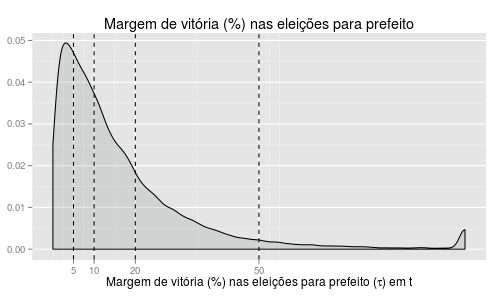
\includegraphics[scale=0.9]{c1g1.png}
	\caption{Distribuição da diferença entre primeiros e segundos colocados nas eleições municipais (1996, 2000, 2004 e 2008)}
	\label{fig:c1g1} 
\end{figure}

Observe-se que não interessa para esta pesquisa o quão bem sucedidos os partidos são nas eleições municipais em geral. O PSDB, por exemplo, venceu 55\% das disputas em que terminou em primeiro ou segundo lugar, enquanto o PT venceu apenas em 47\% das vezes em situações como esta. Uma vez que o objetivo é comparar os casos em que o PSDB venceu com os casos em que o próprio PSDB perdeu, e assim sucessivamente para todos os partidos até para que se obtenha um efeito médio para o conjunto de partidos, as taxas de sucesso individual de cada sigla não importam.

Mais importante do que o desempenho dos partidos nas eleições municipais é a correlação do desempenho com as eleições para os demais cargos estaduais e nacionais. O pressuposto de que existe um conjunto de variáveis não observáveis -- reputação do partido no município, qualidade de suas campanhas e dos candidatos, etc -- implica na existência de correlação positiva entre os votos para prefeito (ou as margens de vitória e derrota de cada partido) e os votos para deputado federal e estadual, senador, governador e presidente. 

A Figura~\ref{fig:c1g2} apresenta gráficos com o desempenho eleitoral para os cargos nacionais e estaduais pelo percentual de votos que o partido obteve nas eleições anteriores para prefeito. Estão incluídos todos os partidos em todos os municípios em que o partido concorreu na eleição municipal dois anos antes, ou seja, contempla o universo dos casos de pares de eleição paras as quais é possível observar os resultados de um partido.

É importante notar que as situações em que os partidos não obtiveram votos para senador, governador ou presidente por não lançarem candidatos estão excluídas. Nestes casos, o ``resultado nulo'' é também produto de outros fatores além daqueles inerentes às disputas eleitorais e sua introdução levaria a resultados inapropriados. Também por esta razão estão excluídas as situações em que houve candidatura única para prefeito, evitando ``bons desempenhos'' artificiais. Por outro lado, parto da premissa de que o partido não receber nenhum voto em algum município para deputado federal ou estadual é uma medida adequada do desempenho do partido, posto que não há restrições ao lançamento de candidaturas para tais cargos. Por fim, no caso específico de senadores, se há dois candidatos do mesmo partido disputando uma eleição plurinominal, os votos dos candidatos são somados e divididos pelo total de votos válidos, uma vez que cada eleitor emite dois votos e o denominador é a soma de todos os votos válidos de todos os eleitores. Apenas no último painel, com dados para as eleições para vereador, que as variáveis dos dois eixos são contemporâneas, ou seja, referem-se à mesma eleição. A linha vermelha é uma reta de regressão que descreve a relação entre as duas variáveis.

\begin{figure}[htp]
	\centering
	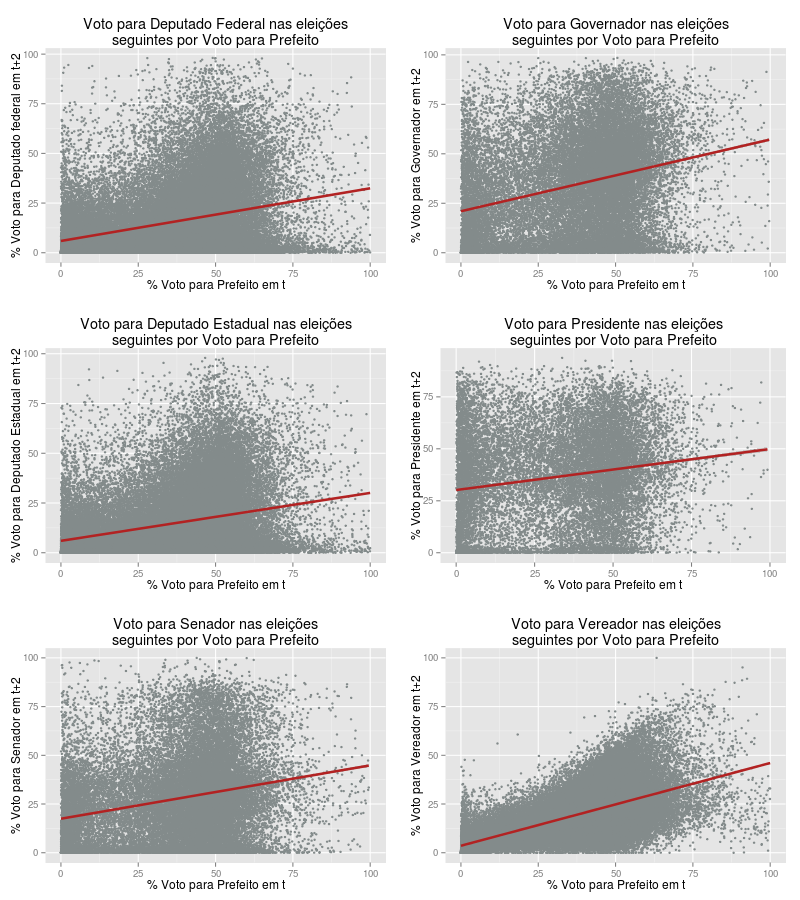
\includegraphics[scale=0.55]{c1g2.png}
	\caption{Voto nas eleições nacionais e estaduais pelo voto para prefeito nas eleições anteriores (pares de eleição 1996-1998, 2000-2002, 2004-2006 e 2008-2010)}
	\label{fig:c1g2} 
\end{figure}

O primeiro aspecto a se observar é que os gráficos da Figura~\ref{fig:c1g2} têm distribuições bastante inusitadas e dispersas, exceto pelo gráfico com dados das eleições para vereador. A relação entre o desempenho para o Legislativo municipal e para prefeitura em uma dada eleição estão altamente correlacionado e há poucos casos que contradizem esta situação. O destino de candidatos a prefeito e a vereador de um partido estão entrelaçados, ainda que seja difícil descrever quais são os fatores que explicam o bom ou o mal desempenho de um partido em uma eleição municipal.

Como $Y_{i}$ e $\tau_{i}$ são, em teoria, funções de um mesmo conjunto de fatores não observáveis, a expectativa é que a relação entre tais variáveis seja positiva. Claramente, a correlação entre o desempenho em eleições subsequentes é positiva e a inclinação da linha vermelha em qualquer um dos gráficos nunca é negativa ou horizontal. Espera-se que os partidos tenham um desempenho melhor para os cargos nacionais e estaduais também nos municípios em que tiveram boa performance dois anos antes. Entretanto, a associação entre desempenho nas eleições para prefeito e a votação nas eleições seguintes é relativamente fraca e há que se chamar atenção para alguns aspectos relevantes nos gráficos da figura.

O principal deles é que as distribuições para os cargos de deputado federal e estadual, semelhantes entre si, são muito diferentes das distribuições para senador, governador e presidente. Nas eleições porporcionais, é bastante comum os partidos terem votação em algum município igual a zero ou muito próxima a zero (pontos próximos ao eixo das ordenadas), mesmo em se tratando de partidos competitivos. No caso das demais eleições, o conjunto de casos próximos com votação próxima a zero é composto pelos candidatos não competitivos. Em uma eleição para presidente, governador e senador, espera-se que os candidatos com chances efetivas de vencer tenham votos em todos os municípios.

Da mesma forma, há menos casos em que o partido tem um bom desempenho nas eleições para a Câmara dos Deputados ou Legislativos estaduais e, simultaneamente, um candidato a prefeito com performance eleitoral muito ruim em relação às demais eleições. Por outro lado, é comum que candidatos à presidência, aos governos estaduais ou ao Senado obtenham bons resultados em municípios em que seus partidos não conseguem lançar candidatos competitivos para a prefeitura.

\begin{figure}[htp]
	\centering
	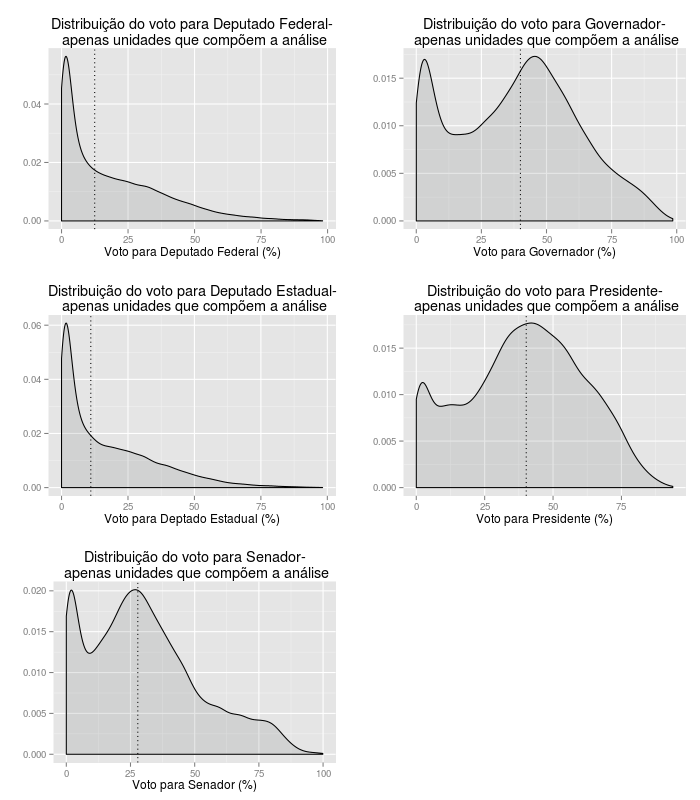
\includegraphics[scale=0.55]{c1g3.png}
	\caption{Distribuição da votação nas eleições nacionais e estaduais para unidades incluídas na análise (1998 a 2010)}
	\label{fig:c1g3} 
\end{figure}

A Figura~\ref{fig:c1g3} apresenta a distribuição das cinco variáveis dependentes adotadas nesta capítulo, ou seja, o percentual de voto para os cinco cargos em disputa nas eleições nacionais e estadual e, diferentemente da Figura~\ref{fig:c1g2}, contém apenas os casos em que o partido $p$ terminou a eleição para prefeito em primeiro ou segundo colocado. Ou seja, uma observação é incluída na distribuição do percentual de votos para deputado federal no município somente se for de um partido que terminou a eleição para prefeito anterior entre os dois primeiros partidos mais bem votados.

A regra eleitoral e as escolhas de como tratar as situações em que o partido não concorreu para prefeitura ou não teve nenhum voto nas eleições seguintes contribuem para explicar tais distribuições. Para os cargos disputados em eleições proporcionais, a distribuição é unimodal, bastante assimétrica e seu pico é deslocado para a esquerda. São raros os casos de partidos que conquistam a maioria dos votos no município, normalmente distribuído entre vários partidos.

As distribuições dos votos para senador, governador e presidente das observações que compõem a amostra, por sua vez, são bastante diferentes. Tais distribuições têm dois picos, um próximo a zero e outro próximo à mediana (linha vertical pontilhada nos gráficos). O primeiro, próximo a zero, é formado pelos candidatos pouco competitivos em eleições majoritárias e, não a toa, na distribuição da votação para presidente a densidade destes casos é menor. O segundo é composto pela votação dos candidatos com chances mais altas de vitória e, portanto, próxima à mediana. Se houvesse apenas dois partidos no Brasil, seria bastante provável que a distribuição das votações para senador, governador e presidente se aproximassem de uma curva normal.

A consequência imediata das distribuições acima observadas é que dispersão de $Y_{i}$ será grande, mesmo próximo à fronteira de atribuição do tratamento definida por $\tau_{i}=0$. Em outras palavras, haverá casos em que a performance eleitoral do partido nas eleições nacionais ou estaduais será baixa mesmo ao selecionar apenas eleições competitivas e definidas por uma margem estreita de votos, em que primeiro e segundo colocados têm desempenhos semelhantes e melhor do que os demais oponentes.

A Figura~\ref{fig:c1g4} ilustra este ponto e contribui para melhor compreender o procedimento analítico da tese. Os quatro gráficos que a compõem são iguais, exceto pelos limites impostos à margem de vitória, representada pelo eixo das abicissas. Em cada um deles, somente os partidos que terminaram a eleição em primeiro ou segundo colocado na competição pela prefeitura foram incluídos. Cada ponto representa um partido ($p$) em um município ($m$) e indica o total de votos recebidos para deputado federal ($Y_{i}$) na eleição $t+2$ (1998, 2002, 2006 ou 2010) pela margem de vitória do partido na eleição para prefeito ($\tau_{i}$) em $t$ (1996, 2000, 2004 ou 2008). Os pontos mais escuros em cada gráfico representam as unidades não tratadas, ou seja, os casos em que o partido perdeu as eleições municipais. Para estas observações $\tau_{i}$ é negativo, variando de 0\% a próximo de -100\%. Os pontos claros, por sua vez, representam os partidos vitoriosos e com $\tau_{i}>0\%$. A linha vermelha no gráfico é uma reta de regressão que descreve a relação entre $Y_{i}$ e $\tau_{i}$ para as unidades não tratadas e a linha azul corresponde à reta das unidades tratadas. Não há sobreposição entre tratados e não tratados, posto que a atribuição do tratamento é uma função determinística da margem de vitória. Gráficos semelhantes para deputado estadual, senador, governador e presidente estão no Anexo da tese.

\begin{figure}[htp]
	\centering
	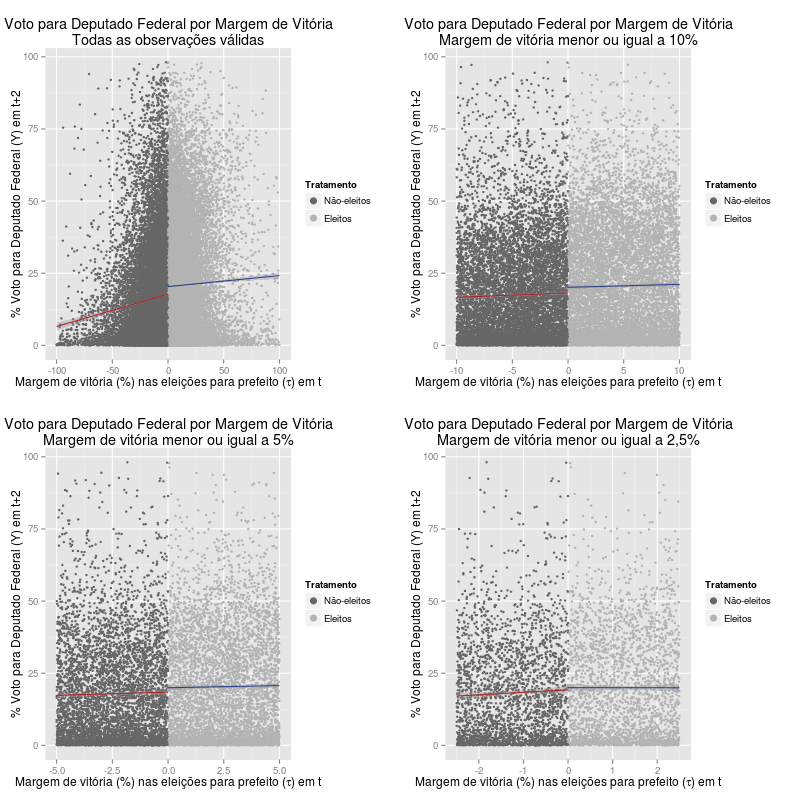
\includegraphics[scale=0.55]{c1g4.png}
	\caption{Voto para Deputado Federal por margem de vitória para prefeito (1996 a 2010)}
	\label{fig:c1g4} 
\end{figure}

A Figura~\ref{fig:c1g4} exemplifica com clareza a estratégia analítica adotada no capítulo e no restante da tese. Em vez de comparar todas as observações e analisar o desempenho para deputado federal entre eleitos e não eleitos, se compara apenas as observações próximas à fronteira de atribuição do tratamento ($\tau_{i}=0$, no centro do gráfico). Quanto menor for a amplitude da margem de vitória, mais bem identificado é o efeito causal.

Note-se que a dispersão de $Y_{i}$ é bastante grande, mesmo quando a margem de vitória é inferior a 2,5\%. Há muitas observações próximas a zero e algumas que chegam a perto de 100\% dos votos válidos para deputado federal. Não é claro, pois, qual é a função de $\tau_{i}$ que melhor descreve a distribuição de $Y_{i}$. Por outro lado, a dispersão é praticamente constante na região de $\tau_{i}$ próximo a zero. As retas que representam cada um dos grupos de tratamento que, no primeiro gráfico, tem inclinação mais acentuada, tendem à horizontalidade quanto menor for a restrição imposta à margem de vitória. Tendo em vista a distribuição conjunta de $Y_{i}$ e $\tau_{i}$ próxima à condição de identificação, não há razões fortes para acreditar que o estimador do efeito causal ($\rho$) por Mínimos Quadrados Ordinários seja viesado. Assim, conforme comentado acima, em alguns momentos da tese será apresentada apenas estimativa de $\rho$ obtida por uma regressão linear local para evitar a apresentação excessiva de informações.

Os gráficos da Figura~\ref{fig:c1g4} contribuem para reforçar a suspeita de que a hipótese deste capítulo -- de que a vitória para prefeitura afeta o resultado nas eleições nacionais e estaduais subsequentes -- está correta. O desnível entre a reta que se ajusta aos pontos de unidades tratadas (azul) e a reta das unidades não tratadas (vermelha) é um indicativo de que o tratamento (vencer as eleições para prefeito) tem efeito. Antes de avançar para a análise, porém, vale a pena observar melhor a relação entre as condições de tratamento -- eleito ou não-eleito -- e o desempenho nas eleições nacionais e estaduais.

\begin{figure}[htp]
	\centering
	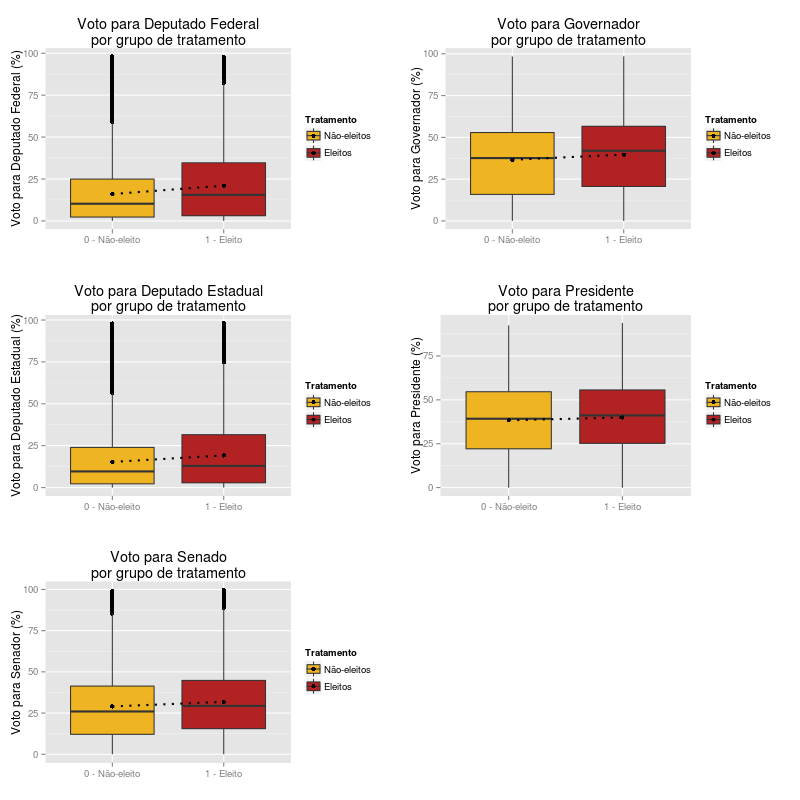
\includegraphics[scale=0.55]{c1g5.png}
	\caption{Voto para Deputado Federal por margem de vitória para prefeito (1996 a 2010)}
	\label{fig:c1g5} 
\end{figure}

Os boxplots da Figura~\ref{fig:c1g5} comparam as distribuições de unidades tratadas e não tratadas para as cinco disputas diferentes. A linha tracejada une as médias dos grupos, que são representadas por um ponto. A inclinação positiva em todos os casos indica que os partidos têm desempenho médio em municípios nos quais governam a prefeitura superior aos municípios em que os partidos perderam a eleição para prefeito anterior e terminaram em segundo lugar. Este resultado descritivo, entretanto, não implica necessariamente em uma relação causal entre vencer a eleição para prefeito e o desempenho posterior, como discutido anterioremente.

As médias entre os grupos são bastante diferentes, bem como as diferenças. Por exemplo, enquanto as médias do percentual de voto para deputado federal para o grupo de eleitos e não eleitos são aproximandamente 20,8\% e 15,8\%, respectivamente, as médias do percentual do voto para presidente são 38,2\% e 39,8\%. Os patamares médios de cada grupo, porém, pouco importam. Apesar das médias serem mais baixas no primeiro caso para os dois grupos, a diferença também é consideravelmente maior e é na diferença em que me concentrarei no restante do capítulo. Dado que as distribuições são semelhantes para tratados e não tratados, não há razões sérias para suspeitar que, uma vez atendida a condição de identificação do desenho de regressão descontínua, os resultados são consequência de distribuições assimétricas. 

Na próxima seção examino com mais cuidado se os requisitos para a estimação do efeito causal por regressão descontínua são atendidos para o problema proposto nesta tese. 

\subsection{Testando a validade do Desenho de Regressão Descontínua: o não-impacto das eleições para prefeito em resultados eleitorais passados}

Um dos principais riscos que desenhos de pesquisa \emph{quasi}-experimentais oferecem é o potencial desequilíbrio em covariáveis entre unidades tratadas e não tratadas. Se estas covariáveis estiverem correlacionadas com a variável resposta ($Y_{i}$) e não forem incluídas no modelo como variáveis de controle, então o efeito estimado do tratamento será viesado. Em particular, isto é o que acontece quando tais covariáveis não são observáveis.

Por exemplo, se os partidos vitoriosos têm sistematicamente campanhas mais caras ou um histórico eleitoral no município melhor do que partidos derrotados, e nenhum destes fatores forem controlados ou não forem observáveis, a diferença no desempenho eleitoral futuro ($Y_{i}$) entre os grupos de tratamento não necessariamente é resultado do tratamento.

O problema operacional central em um desenho de regressão descontínua é garantir que as estimativas sejam obtidas apenas a partir de observações suficientemente próximas da fronteira, subconjunto para o qual a condição de identificação dos efeitos causais é válida. Logo, em um RDD, espera-se que as unidades próximas à fronteira ($\Delta$ próximo a zero) sejam semelhantes entre si exceto, obviamente, na variável resposta ($Y_{i}$).

Portanto, no caso de um RDD em que o tratamento é vencer as eleições majoritárias, espera-se que as unidades tratadas e não tratadas que estejam próximas à fronteira não sejam diferentes quanto aos aspectos da competição eleitoral não afetados pelo tratamento, ou seja, quanto a fatores não observáveis.

Há algumas maneiras de testar se essa condição é válida. Uma delas é analisar se a vitória para prefeito tem impacto em fenômenos que ocorreram antes ou simultaneamente à eleição municipal (aqui representadas por $O_{i}$). Por exemplo, as eleição para prefeito e vereador ocorrem no mesmo dia. Assim, apesar da votação para prefeito e vereador estarem bastante correlacionadas, não deve haver efeito causal da vitória para prefeito na votação para vereador do partido. O bom ou mal desempenho em ambas as votações deve ser explicado por outros fatores ($A_{i}$), normalmente desconhecidos ou para os quais não temos mais do que pistas teóricas. Mas certamente a vitória para prefeito não pode impactar nos votos para vereador do partido. 

Logo, antes de produzir estimativas dos efeitos do tratamento, é prudente observar se os grupos de tratamento e controle são semelhantes em relação a variáveis que não deveriam, por construção, ser afetadas pelo próprio tratamento. Vencer as eleições para prefeito não deve ter impacto nos resultados eleitorais passados do partido, não pode afetar o resultado das eleições para vereador que ocorrem no mesmo dia e não pode ter efeito nas contas de campanha da própria eleição para prefeito ou nas transferências que o município recebeu do governo federal no passado. $O_{i}$ pode explicar $d_{i}$, mas o contrário é necessariamente falso.

Nesta seção examino empiricamente se a vitória para prefeito ($d_{i}$) tem efeito nas variáveis passadas ou contemporâneas às eleições municipais ($O_{i}$). Como este efeito é necessariamente falso, sua existência indica o desequilíbrio dos grupos de tratamento em covariáveis. Mesmo havendo correlação positiva entre $\tau_{i}$, $O_{i}$ e $Y_{i}$, o efeito estimado deve ser nulo.

Como em cada município há um vencedor e pelo menos um perdedor, por construção, não há desequilíbrio entre os grupos de tratamento quanto às características médias dos municípios (representadas a partir daqui por $M_{i}$). Isso é válido, porém, apenas quando a ausência de candidatos do partido com votos no município é equivalente a ter desempenho eleitoral nulo, como ocorre nas eleições para deputado federal e deputado estadual. Porém, na análise do impacto do tratamento na performance para senador, governador e presidente há municípios que, para algumas eleições, estão presentes em apenas uma vez no conjunto de observações válidas, ou seja, apenas em um dos grupos de tratamento. Pode ocorrer, por exemplo, do grupo de tratados ser composto por municípios de tamanho, renda per capita ou dependência de transferências federais e estaduais diferente dos municípios no grupo de não tratados. Logo, além de examinar se há equilíbrio entre tratados e não tratados quanto a resultados eleitorais passados ($O_{i}$), para parte das análises deste capítulo também é necessário verificar se há equilíbrio entre os grupos também quanto às características médias dos municípios ($M_{i}$).

\begin{figure}[htp]
	\centering
	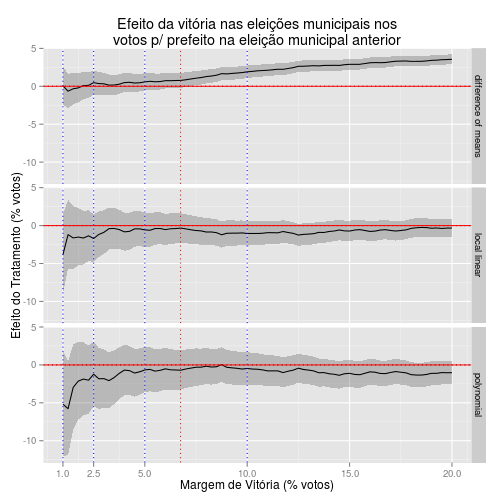
\includegraphics[scale=0.55]{c1g6.png}
	\caption{Efeito do Tratamento no Voto para Prefeito na \textbf{eleição municipal anterior} por margem de vitória para prefeito (1996 a 2008)}
	\label{fig:c1g6} 
\end{figure}

A Figura~\ref{fig:c1g6} apresenta o efeito do tratamento ($\rho$) nos votos para prefeito na eleição municipal anterior ($O_{i}$) por margem de vitória. Cada gráfico apresenta o efeito estimado por método de estimação: diferença de médias, regressão linear ou regressão polinomial, respectivamente. A linha escura representa o efeito estimado selecionando as observações por intervalo de margem de vitória. Por exemplo, quando a margem de vitória indicar 15\%, significa que o efeito do tratamento ($\rho$) foi estimado utilizando todas as observações cujo módulo da margem de vitória ($\Delta$) foi menor que 15\%, ou seja, todos os casos em que o partido foi derrotado ou vitorioso por uma margem menor ou igual a essa. O valor do margem de vitória no gráfico representa o limite superior de $\Delta$ para incluir uma observação, mas, para simplificar o texto, ``limite superior da margem de vitória'' será simplesmente ``margem de vitória''.

A área cinza que acompanha a linha é o intervalo de confiança de 95\% da estimativa. As linhas azuis verticais são pontos de referência: margens de vitória de 1\%, 2,5\%, 5\% e 10\%. A linha vermelha vertical indica a \textit{optimal bandwidth} ($\Delta_{IK}$) calculada pelo método de \citet{Imbens2011}. A reta vermelha horizontal nada mais é do que o ponto em que o efeito é zero ($\rho=0$).

Por exemplo, no gráfico onde se lê \textit{local linear} se produziu uma regressão linear para estimar o coeficiente da variável de tratamento $d_{i}$ sobre $Y_{i}$ (e o seu respectivo intervalo de confiança de 95\%) para todas as observações cujo módulo da margem de vitória ($\Delta$) é menor do que o valor do eixo das abscissas. O gráfico é a combinação de 80 regressões lineares, um para cada conjunto de observações com margem de vitória menor do que um determinado valor no intervalo de 0\% a 20\%, com intervalos de 0,25\% entre si. Assim, ao escolher uma margem de vitória de 20\%, todas as eleições que foram decididas por este percentual ou menos são selecionadas. O efeito estimado por diferença de médias, neste ponto, é de aproximadamente 3,6\% (extremidade direita da linha escura). Para uma margem de 5\% o efeito estimado é próximo a zero (0,6\%).

É fácil notar para uma margem qualquer escolhida se o efeito estimado é diferente de zero: basta observar se a área cinza (intervalo de confiança do estimador) coincide com a reta vermelha horizontal ($\rho=0$, ou seja, efeito do tratamento nulo). Se não coincidir, é possível refutar a hipótese nula de que o tratamento não tem efeito, podendo ser positivo (parte superior do gráfico, acima da linha vermelha) ou negativo (parte inferior do gráfico, abaixo da linha vermelha).

Como era de se esperar, o resultado para prefeito em uma eleição não têm impacto no resultado nas eleições anteriores, não importando a maneira pela qual medimos esse efeito. O efeito estimado é estatisticamente diferente de zero apenas no primeiro gráfico do painel e para margens de vitória superiores a 7\%. Este resultado é particularmente importante para prosseguir com a análise dos efeitos causais da vitória para prefeito em outras variáveis. Das várias medidas possíveis de $O_{i}$, o voto na própria eleição anterior para prefeito é certamente uma das mais adequadas em virtude da correlação com $\tau_{i}$ e com os demais fatores não observáveis $A_{i}$.

\begin{figure}[htp]
	\centering
	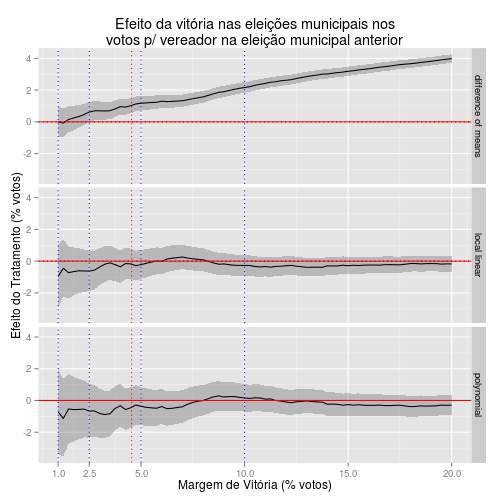
\includegraphics[scale=0.55]{c1g7.png}
	\caption{Efeito do Tratamento no Voto para Vereador na \textbf{mesma eleição municipal} por margem de vitória para prefeito (1996 a 2008)}
	\label{fig:c1g7} 
\end{figure}

A Figura~\ref{fig:c1g7} apresenta resultados semelhantes, com a diferença que $O_{i}$ é agora o desempenho do partido nas eleições para vereador na mesma eleição municipal, ou seja, no mesmo momento em que tratamento e controle são atribuídos. Como se observou na Figura~\ref{fig:c1g2}, o voto para vereador e para prefeito estão bastante correlacionados. Não por acaso: candidatos a prefeito e vereador de um partido fazem campanhas no mesmo palanque, se apoiam mutuamente, dividem recursos e estão sujeitos às mesmas condições eleitorais (mesma reputação do partido naquele município/eleição, por exemplo). Novamente, a expectativa de um resultado nulo se confirma. Entrentanto, no primeiro painel, vemos que há efeito positivo e estatisticamente diferente de zero no caso para margens superiores a 2.5\%.

Há algumas considerações e observações importantes a se fazer sobre as Figuras~\ref{fig:c1g6} e~\ref{fig:c1g7}. A primeira delas é que a diferença de médias é um estimador do efeito do tratamento bastante mais sensível à margem de vitória. Como a expectativa é que $\tau_{i}$ e $Y_{i}$ estejam correlacionados aos mesmos fatores não-observáveis ($A_{i}$), também se espera que haja correlação entre o efeito causal ($\rho$) e a margem de vitória. Ainda assim, o padrão descrescente do efeito em relação à margem, mesmo esperado, é encontrado em todos os outros testes produzidos com diferenças de médias e coloca em dúvidas a validade do estimador para uma margem de vitória arbitrariamente escolhida. Basta observar que a estimativa pontual de $\rho$ troca de sinal ao se reduzir a margem.

As outras duas maneiras de estimar $\rho$ -- como uma descontinuidade em uma função linear ou polinomial -- sofrem menos com a variação de $\tau_{i}$. A introduzir $\tau_{i}$ como controle na estimação de $\rho$, as unidades são comparadas também levando em conta sua distância do ponto de corte $\tau_{i}=0$ e a inclinação observada nas estimativas por diferença de médias desapareçam.

Entretanto, como se observa rapidamente, os desvios padrão são bastante maiores e bastante instáveis quanto menor for a margem e, portanto, o número de observações. A variação é especialmente grande quando $\Delta$ é menor que 5\%. Particularmente, este primeiro resultado e a observação empírica dos demais que seguem sugerem que uma das combinações mais confiáveis para estimar o efeito causal para o problema em questão é a utilização de uma função linear e margens iguais ou menores que 5\%. Quando, por parcimônia, não for possível apresentar os resultados completos, concentrarei a análise ao intervalo entre 0\% e 5\%, com especial atenção ao ponto em que $\Delta=2,5\%$.

Esses dois primeiros resultados tornam bastante seguro afirmar que, pelo menos para estimativas do efeito causal em que a variação de $\tau_{i}$ é controlada ou para margens menores que 2,5\%, não há desequilíbrio entre grupos de tratamento e controle. Qualquer outra variável escolhida para medir $O_{i}$ é, pela construção do problema, menos interessante do que o resultado passado nas eleições para prefeito e/ou o resultado contemporâneo nas eleições para vereador. Porém, antes de avançar, convém observar mais alguns testes utilizando como $O_{i}$ a própria variável dependente $Y_{i}$ defasada em uma eleição e as características dos municípios.

\begin{figure}[htp]
	\centering
	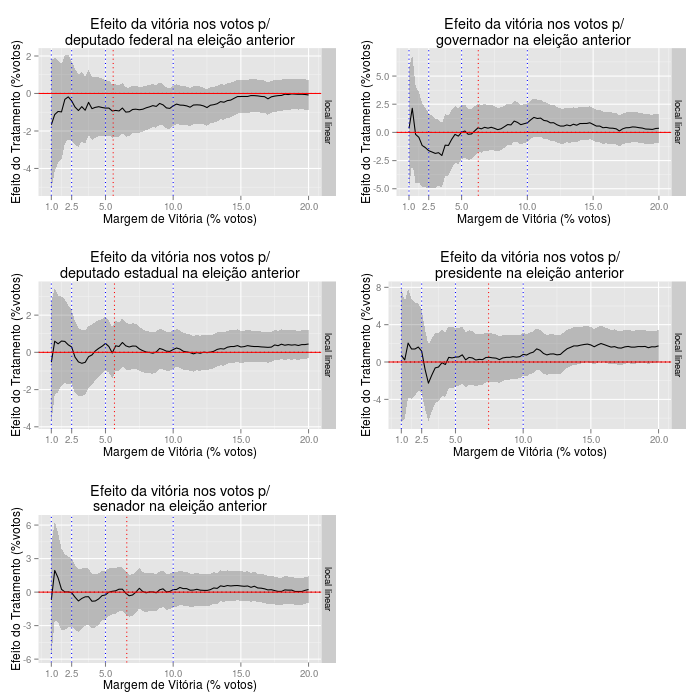
\includegraphics[scale=0.60]{c1g8.png}
	\caption{Efeito do Tratamento no Voto para Todos os Cargos na \textbf{eleição anterior} por margem de vitória para prefeito (1994 a 2008)}
	\label{fig:c1g8} 
\end{figure}

Os gráficos da Figura~\ref{fig:c1g8} trazem as estimativas dos efeitos do tratamento para os cinco cargos em competição nas eleições nacionais e estaduais anteriores. Novamente, em nenhum dos casos há efeito algum do tratamento sobre o desempenho do partido no passado. Há razões para acreditar, portanto, que os grupos estão devidamente balanceados e, uma vez atendida a condição de identificação necessária em um RDD, os resultados da análise não são consequência da presença de fatores não identificados.

Por fim, para as situações nas quais há exclusão de observações de partidos sem candidatos aos cargos de senador, governador ou presidente, testo se não há diferenças relevantes entre os grupos de tratamento em relação às características médias do município (aqui representadas por $M_{i}$). A principal característica municipal em que há risco de desequilíbrio é o número de habitantes, que, por sua vez, está correlacionado ao tamanho do eleitorado e a diversas outras características do município. As observações tratadas provêm de municípios de mesmo tamanho que as observações não tratadas? Como se observa nos gráficos da primeira coluna da Figura~\ref{fig:c1g9}, não há razões para acreditar em desequilíbrio em relação a esta variável para nenhum dos cargos quando a margem de vitória se aproxima de zero.

O mesmo procedimento é repetido para outras duas características dos municípios ($M_{i}$): o PIB municipal \textit{per capita}; e o grau de dependência da prefeitura em relação a transferências de outros governos, medida como a razão entre as receitas de transferências e o total de receitas orçamentárias do município. No primeiro caso, pretende-se eliminar a hipótese de que os resultados são condicionados por municípios tratados terem renda mais alta do que os não tratados e vice-versa. No segundo, o objetivo é evitar que resultados provenham de desequilíbrio entre grupos de tratamento quanto à capacidade do prefeito em produzirr políticas com recursos próprios e/ou quanto à dependência de outros níveis de governo e, portanto, de outros atores políticos. A Figura~\ref{fig:c1g9} mostra que, também para estas duas características, tratados e não tratados são bastante equivalentes.

\begin{figure}[htp]
	\centering
	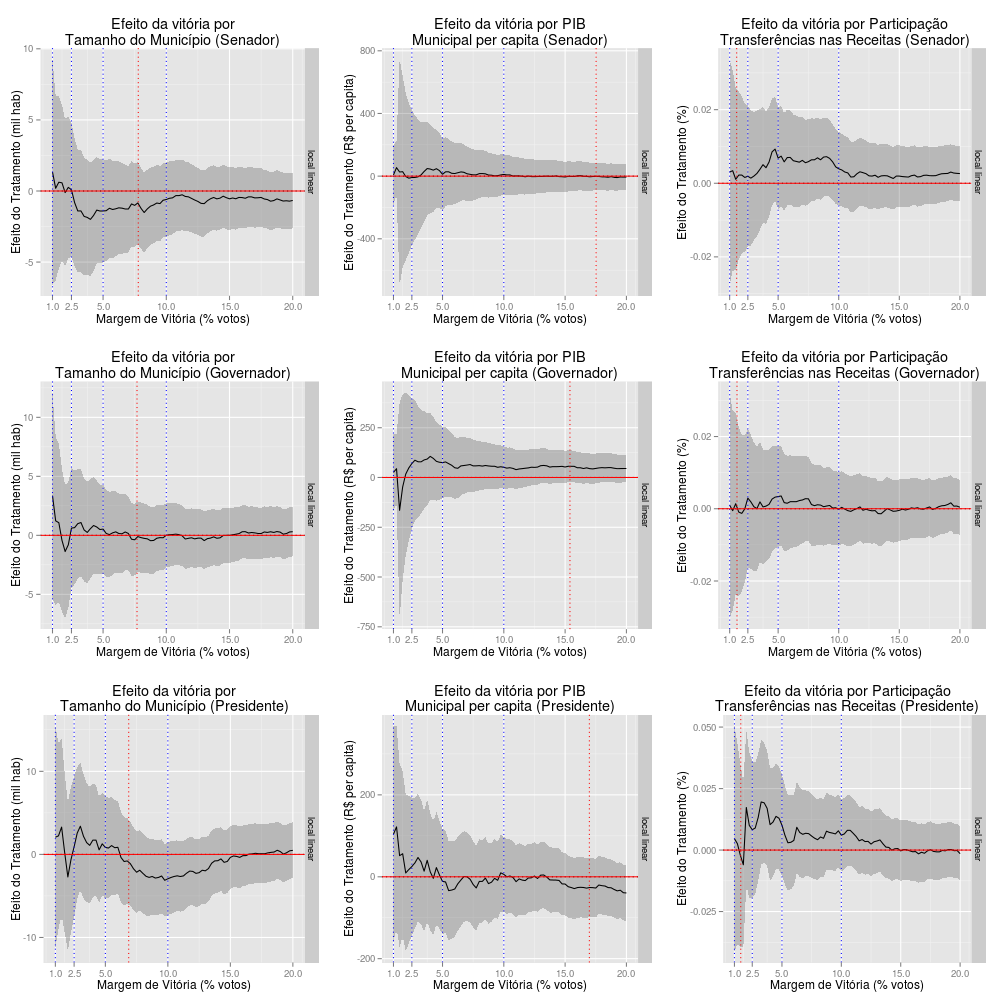
\includegraphics[scale=0.48]{c1g9.png}
	\caption{Efeito do Tratamento no Voto para características municipais no \textbf{ano da eleição municipal} por margem de vitória para prefeito (1996 a 2008) - subconjuntos de dados para análise de senador, governador e presidente}
	\label{fig:c1g9} 
\end{figure}

Nos Capítulos~\ref{cap:emendas} e ~\ref{cap:mecanismos} será preciso apresentar testes para outros subconjuntos de observações e variáveis. O objetivo e o procedimento da análise continuará o mesmo. Por enquanto, porém, já há evidências suficientes para afastar os riscos de que os resultados apresentados neste primeiro capítulo derivam de desequilíbrio entre os diferentes grupos de tratamento. Como se demonstrou acima, quando procuramos uma descontinuidade provocada pelo tratamento em variáveis cuja ocorrência é anterior ou contemporânea à própria atribuição do tratamento nenhum efeito é encontrado. Os resultados apresentados na seção seguinte não derivam, pois, de desequilíbrios nos grupos de tratamento\footnote{O Capítulo~\ref{cap:financiamento} retoma o tema do desequiblíbrio entre os grupos de tratados e não tratados e apresenta problemas inicialmente não discutidos nesta seção. Como se observará adiante, há uma variável para a qual o desequilíbrio entre tratados e não tratados é mais sério: as receitas de campanha para prefeito. Sistematicamente, partidos vitoriosos arrecadaram mais do que partidos derrotados, mesmo quando são comparados apenas os casos nos quais a margem de vitória tende a zero. O Capítulo~\ref{cap:financiamento} trata apenas deste assunto e revê os resultados dos três primeiros capítulos à luz deste problema.}.

\section{O impacto das eleições para prefeito no Brasil: eleições para deputado federal e estadual}

Objetivo deste capítulo, e primeiro propósito da tese, é avaliar o impacto das eleições para prefeito no desempenho do partido nas eleições para os demais cargos estaduais e federais. A hipótese central é que o partido tem resultado eleitoral superior para os cargos de deputado federal, deputado estadual, senador e presidente em municípios nos quais venceu as eleições anteriores para prefeito do que em municípios nos quais perdeu a eleição. O período de análise contempla as eleições de 1996 a 2010.

Na Figura~\ref{fig:c1g5} vimos que, na média, os partidos têm desempenho superior em municípios nos quais venceram a disputa para prefeitura, para qualquer um dos cinco cargos. Entretanto, não sabemos se há impacto causal de vencer as eleições para prefeito ($d_{i}$) na performance eleitoral do partido na eleição seguinte, pois tanto a variável que define o resultado das eleições para o Executivo municipal ($\tau_{i}$) quanto o desempenho nacional e estadual do partido, $Y_{i}$, são resultados de um mesmo conjunto de fatores não observáveis ($A_{i}$). A adoção de um desenho de regressão descontínua tem o propósito de identificar corretamente o efeito de $d_{i}$ em ($Y_{i}$).

Nesta seção apresento os resultados e sua respectiva análise. Os primeiros resultados tratam apenas dos cargos para deputado federal e deputado estadual. Além de testar a hipótese principal, exploro uma série de variações desta hipótese para contemplar os efeitos heterogêneos dos resultados e examinar as potenciais diferenças entre eleições, partidos, contextos políticos locais e características dos municípios. A seguir, repito o procedimento para os demais cargos, senador, governador e presidente. Há razões teóricas e práticas para separar os resultados desta maneira. Do ponto de vista teórico, as análises sobre a política brasileira dão atenção especial para a relação entre os parlamentares e os governos locais. Os candidatos às eleições proporcionais dependem  da construção e manutenção de bases eleitorais, enquanto candidatos aos cargos do Executivo ou ao Senado contam com maior exposição televisiva e campanhas mais caras para poderem se eleger. Do ponto de vista prático, o Capítulo~\ref{cap:emendas} trata apenas da relação de prefeitos com deputados federais e, por esta razão, convém também separar os resultados deste capítulo.

\subsection{O impacto das eleições para prefeito no Brasil: eleições para deputado federal e estadual para o período 1996-2010}

Uma das consequências da adoção de eleições proprocionais no Brasil é que virtualmente todos os partidos participam da competição por vagas na Câmara dos Deputados e Assembléias Legislativas. São raros os casos de diretórios estaduais de partidos que não lançam candidatos para deputado federal ou estadual e tais casos estão restritos aos menores partidos. Em 1998 o Brasil teve 3.417 candidatos a deputado federal e 10.051 candidatos a deputado estadual; em 2010 estes números saltaram para 6.015 e 14.382 candidatos, respectivamente.

Há graus bastante variados de sucesso entre os partidos ao longo do tempo nas eleições legislativas, mas a consequência imediata de tamanha dispersão é que a maioria dos partidos recebe votos em todos ou quase todos os municípios do país. Para os propósitos da tese, interessa apenas saber se a fortuna eleitoral dos candidatos de uma agremiação partidária é também resultado da vitória nas eleições para prefeito anteriores, controlando os demais aspectos. O fato dos partidos competirem livremente em todo o território nacional contribui para a análise. Cabe notar que, uma vez que as barreiras de competição nestas eleições são baixas e o componente estratégico do lançamento de candidaturas reside na formação de coligações e não na escolha de cabeças de chapa, é razoável assumir que um partido que decidiu não competir tinha expectativa de voto nula ou quase nula.

A Figura~\ref{fig:c1g10} apresenta o efeito do tratamento ($\rho$) nos votos para deputado federal e estadual ($Y_{i}$) seguintes por intervalo de margem de vitória ($\tau_{i}$). Tal como na seção anterior, cada gráfico apresenta o efeito estimado por métodos de estimação distintos: diferença de médias, regressão linear ou regressão polinomial, respectivamente. Os gráficos à esquerda trazem o resultado para deputado federal. Os gráficos à direita o resultado para os candidatos ao Legislativo estadual. A linha escura representa o efeito estimado selecionando as observações por margem de vitória. A área cinza que acompanha a linha é o intervalo de confiança de 95\% da estimativa. As linhas azuis verticais são pontos de referência: margens de vitória de 1\%, 2.5\%, 5\% e 10\%. A linha vermelha vertical indica a \textit{optimal bandwidth} ($\Delta_{IK}$) calculada pelo método de \citet{Imbens2011}. A reta vermelha horizontal nada mais é do que o ponto em que o efeito é zero ($\rho=0$).

\begin{figure}[htp]
	\centering
	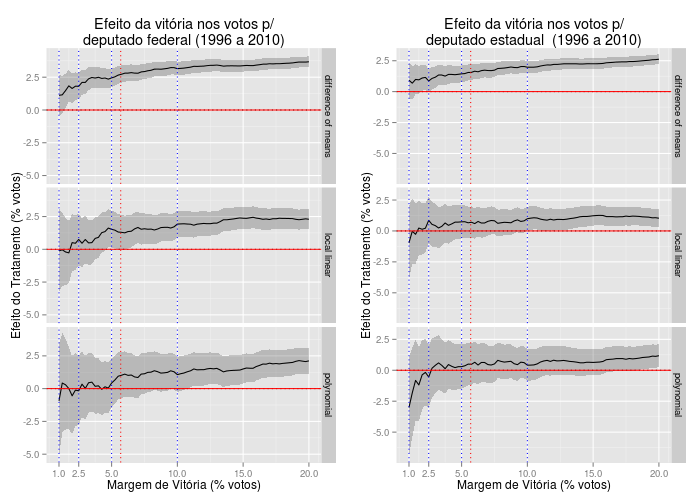
\includegraphics[scale=0.55]{c1g10.png}
	\caption{Efeito do Tratamento no Voto para Deputado Federal e Deputado Estadual nas eleições seguintes por margem de vitória nas eleições para prefeito (1996 a 2008)}
	\label{fig:c1g10} 
\end{figure}

Tanto para deputado federal quanto para deputado estadual só é possível encontrar efeito do tratamento diferente de zero quando $\rho$ é uma diferença de média simples entre o desempenho nas eleições proporcionais em municípios em que o partido perdeu e o desempenho nos municípios em que o partido venceu a disputa pela prefeitura. Adotando a margem de vitória de 2,5\% como referência, temos que o partido recebe, em média, 1,8\% a mais de votos para deputado federal e 0,86\% a mais dos votos para deputado estadual em municípios em que venceu as eleições municipais do que em municípios em que foi derrotado.

Este resultado, porém, é bastante frágil e pouco confiável. Quando se estima o impacto causal de vencer as eleições como descontinuidade em uma função linear, apenas no intervalo entre 5\% e 10\% de margem de vitória há alguma evidência de que o efeito é diferente de zero. Com a adoção de uma função polinomial, o resultado desaparece por completo. Apenas a partir deste primeiro resultado, seria pouco prudente sugerir que há impacto das eleições para prefeito no desempenho do partido nas disputas para a Câmara dos Deputados e Assembléias Legislativas.

\subsection{O impacto das eleições para prefeito no Brasil: eleições para deputado federal e estadual por partido}

O efeito apresentado na Figura~\ref{fig:c1g10}, entretanto, é o efeito médio para todas as eleições em análise, partidos, contextos municipais e condições de disputas. Ao agrupar eleições e partidos assumo, por exemplo, que o efeito é homogêneo ao longo do tempo e constante para todos os contextos municipais. E se houve mudança na capacidade dos partidos se articularem ao longo do tempo? Há diferenças entre prefeitos reeleitos e novos prefeitos?


\begin{figure}[htp]
	\centering
	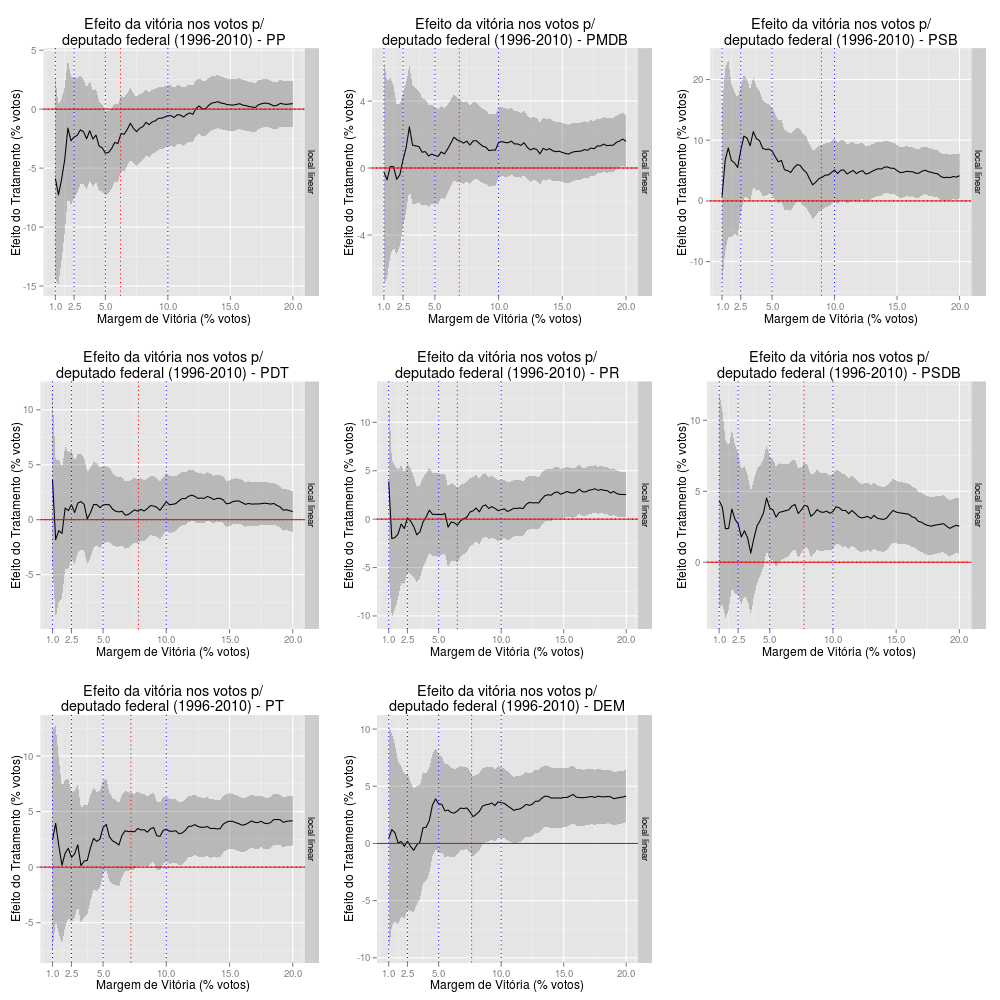
\includegraphics[scale=0.5]{c1g11.png}
	\caption{Efeito do Tratamento no Voto para Deputado Federal nas eleições seguintes por margem de vitória nas eleições para prefeito (1996 a 2008) por partido}
	\label{fig:c1g11} 
\end{figure}

Cada um dos gráficos da Figura~\ref{fig:c1g11} apresenta o resultado por partido político para as eleições para deputado federal\footnote {Por parcimônia, o gráfico inclui apenas os resultados calculados como descontinuidade em uma função linear. Os demais gráficos, com a estimativa por diferença de médias ou como descontinuidade em um função linear, estão no Anexo da tese.}. Os resultados mostram que os partidos são diferentes quanto à capacidade de coordenação entre prefeitos e candidatos a deputado federal, ainda que a maioria dos resultados não sejam diferentes de zero. Aparentemente, PSB e PSDB são partidos para os quais há algum evidência de coordenação durante o período 1996 e 2010. PP, por outro lado é um dos partidos com baixo grau de coordenação ao ponto de haver evidência de que o partido tem desempenho inferior nos municípios nos quais venceu as eleições municipais. PDT, PT e PR são os partidos com menores número de primeiros e segundos lugares em eleições municipais e não é possível encontrar resultados positivos para tais partidos. Por outro lado, PMDB e DEM têm resultados nulos mesmo representando um número grande de observações incluídas na análise.

Na Figura~\ref{fig:c1g12} o procedimento é repetido e são apresentados os efeito estimado do tratamento nos votos para deputado estadual por partido. Basicamente, os resultados para deputado estadual são nulos para todos os partidos com a exceção do PSB.

\begin{figure}[htp]
	\centering
	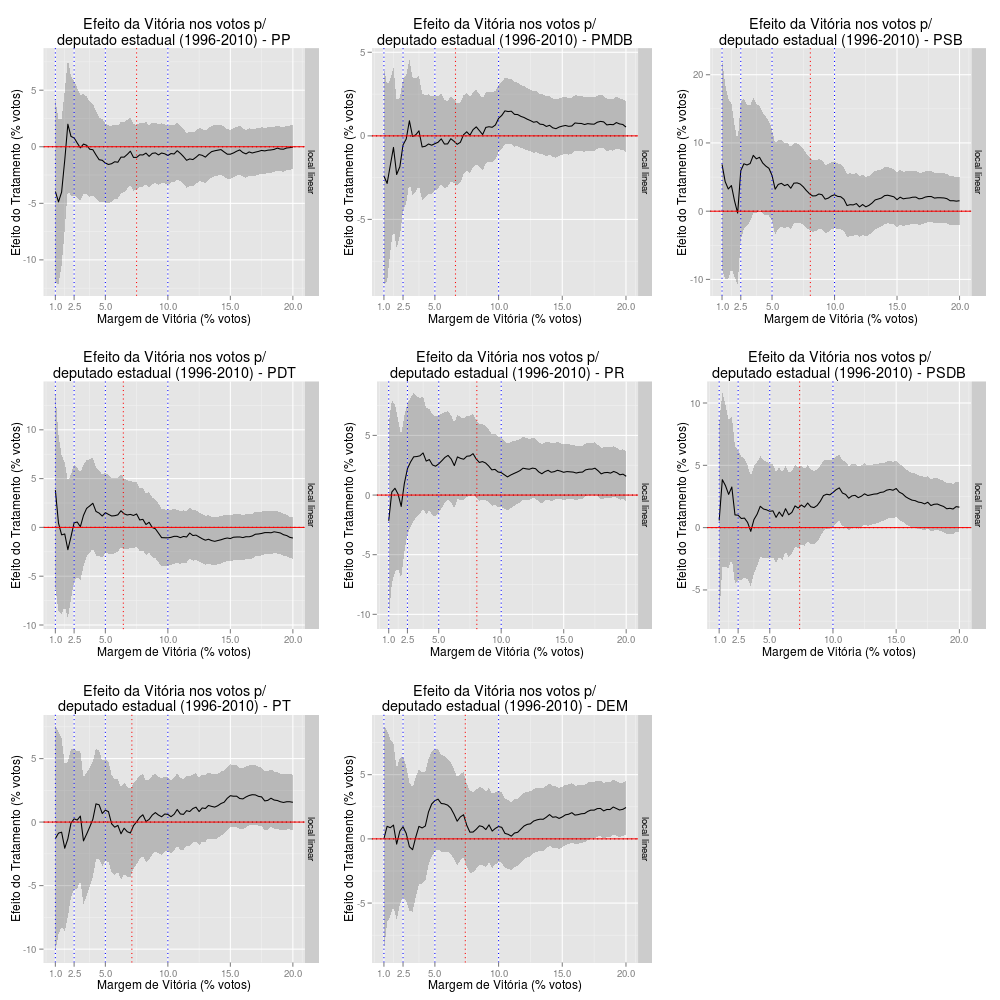
\includegraphics[scale=0.48]{c1g12.png}
	\caption{Efeito do Tratamento no Voto para Deputado Estadual nas eleições seguintes por margem de vitória nas eleições para prefeito (1996 a 2008) por partido}
	\label{fig:c1g12} 
\end{figure}

Um cuidado importante a se tomar é que os partidos provavelmente não têm um único padrão ao longo dos 14 anos incluídos na análise. Alguns partidos como o DEM, por exemplo, começaram a amargar diversas derrotas para os Legislaticos e nos municípios enquanto o PT passou a consquistar um número maior de prefeituras. Vamos examinar a seguir as diferenças entre os pares de eleição incluídos na análise. Infelizmente é muito difícil combinar as duas dimensões (tempo e partido) na análise, posto que cada subconjunto teria um número pequeno de observações.

\subsection{O impacto das eleições para prefeito no Brasil: eleições para deputado federal e estadual para o período 2008-2010}

Em cada um dos gráficos da Figura~\ref{fig:c1g13} apresento os resultados por par de eleições municipais e eleições legislativas nacionais/estaduais. Claramente, há padrões muito diferentes entre anos. Quando observamos em conjunto os seis gráficos com resultados para os dois cargos e para os pares de eleições 1996-1998, 2000-2002 e 2004-2006, e consideramos apenas o intervalos de $\Delta \leq 10\%$, o efeito estimado é, na maior parte das situações, negativo e quase em nenhum momento diferente de zero. Por outro lado, há um claro impacto da vitória nas eleições de 2008 no voto para deputado federal em 2010 e o intervalo de confiança de 95\% cruza a linha vermelha apenas nas menores margens. As estimativas por diferença de médias, omitidas e apresentadas no Anexo, corroboram este resultado. Tomando novamente $\Delta \leq 2,5\%$ como referência, o efeito estimado da vitória no município deste impacto é $\rho=3,4\%$ nos votos do partido para deputado federal nas eleições seguintes.

\begin{figure}[htp]
	\centering
	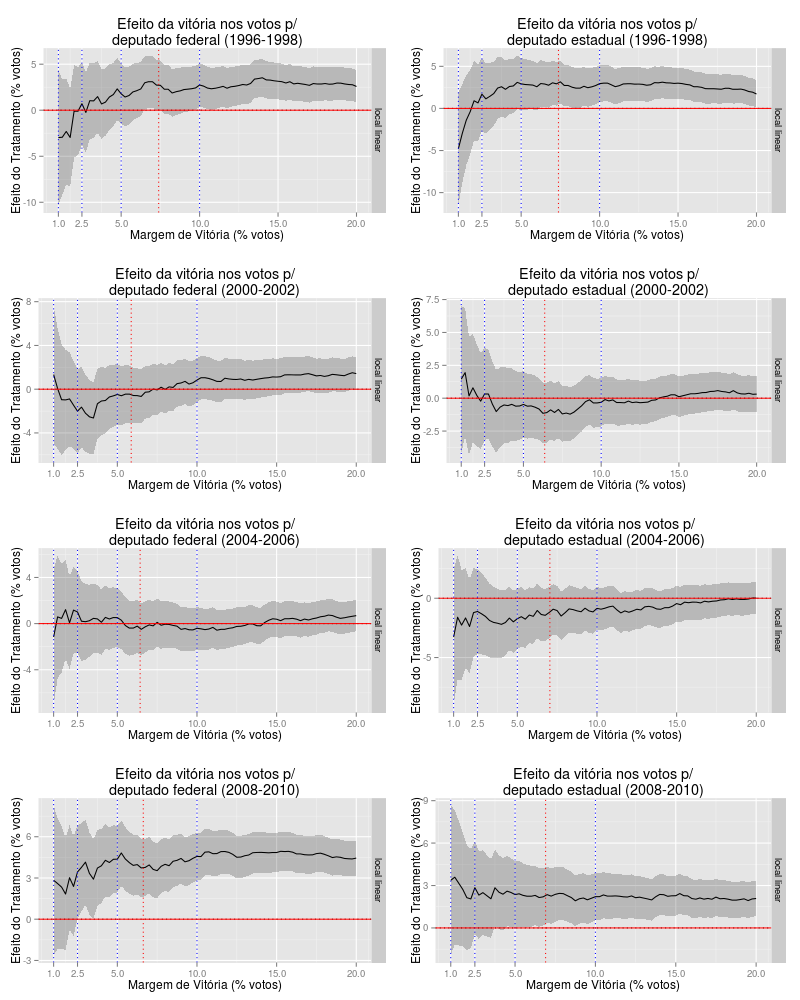
\includegraphics[scale=0.55]{c1g13.png}
	\caption{Efeito do Tratamento no Voto para Deputado Federal e Deputado Estadual nas eleições seguintes por margem de vitória nas eleições para prefeito por par de eleição}
	\label{fig:c1g13} 
\end{figure}

As diferenças entre o período de 1996-2006 e 2008-2010 também aparecem no caso de deputados estaduais. O impacto estimado, porém, e ligeiramente inferior ao de deputados federais e resiste um pouco menos à restrição de observações por margem de vitória. No ponto de referência $\Delta \leq 5\%$, o zero não está contido no intervalo de confiança de 95\% e o impacto estimado da vitória nas eleições para prefeito é de aproximadamente $\rho=2,9\%$ nos votos do partido na próxima eleição para deputado estadual. Em 1996-1998, há um efeito ligeiramente positivo próximo da região em que $\Delta \leq 10\%$. Entretanto, a aproximação de $\Delta$ a zero rapidamente torna o efeito nulo e inverte o sinal da estimativa.

Os resultados por período, indicam, portanto, um comportamento variante dos partidos ao longo do tempo. Há três hipóteses -- não testáveis no escopo desta pesquisa -- que poderiam explicar o padrão encontrado. No período 2000-2004 aproximadamente um quinto dos prefeitos trocam pelo menos uma vez de partido ao longo do mandato \footnote{fonte: elaboração própria a partir de dados de candidaturas e filiação partidária do TSE}. A hipótese central deste capítulo é composta por duas condições: prefeitos são capazes de mobilizar eleitores e prefeitos apoiam preferencialmente candidatos de seu próprio partido. Se prefeitos trocam de partido com frequência, a segunda condição pode não ser satisfeita. Em 2007 o Supremo Tribunal Federal julgou os mandados de segurança propostos por partidos que demandavam o mandato de parlamentares que haviam trocado de partido. A decisão do STF se estendeu não apenas aos cargos disputados em eleições proporcionais, mas também àqueles disputados em eleições majoritárias, incluindo prefeitos. Assim, a primeira hipótese para a existência de resultado positivo a partir de 2008 é que prefeitos deixaram de migrar e, assim, passaram a buscar coordenação dentro dos partidos, apoiando nas eleições nacionais e estaduais candidatos da agremiação pela qual foram eleitos.

A migração de prefeitos pode ser um fator importante. Entretanto, é preciso lembrar que a grande maioria dos prefeitos que migram o fazem apenas no terceiro ano de mandato, ou seja, após as eleições nacionais e estaduais. E se simplesmente prefeitos não forem capazes de mobilizar votos para outros candidatos? De 1996 a 2010 as prefeituras brasileiras tiveram seu papel na provisão de serviços públicos ampliadas e, relativamente, têm mais autonomia do que tinham no começo da década de 1990. Logo, a segunda hipótese é que o papel dos prefeitos como atores políticos se fortaleceu e ampliou a capacidade dos mandatários municipais influenciarem o voto dos eleitores de sua localidade.

Por fim, a mudança do padrão ao longo do tempo pode simplesmente ser resultado de um processo mais amplo de amadurecimento da democracia brasileira e consolidação do sistema partidário. A volatilidade entre eleições tem diminuído; há repetição de disputas e maior previsibilidade nas candidaturas e nos resultados eleitorais; e já houve tempo suficiente para que mais de um partido governasse prefeituras, estados e união e para que a reputação de partidos no eleitorado se consolidasse. Todos esses fatores contribuem para um quadro partidário mais estável e, consequentemente, para tornar mais claro o vínculo organizacional entre prefeitos e demais atores políticos e também para que os esforços de coordenação dentro das organizações partidárias sejam eleitoralmente recompensados.

E se tais hipóteses forem falsas, o resultado encontrado se dever ao fato de 2008 ser uma eleição atípica e com efeitos do da vitória eleitoral obtidos por mero acaso? Infelizmente, apenas com a realização de novas eleições (ou pelo menos ao final de 2014) será possível responder a esta pergunta com um pouco mais de segurança. Como uma série de fatores precisariam operar simultaneamente para que o acaso produzisse o resultado -- por exemplo, parte significativa os partidos simultaneamente se coordenarem internamente e os prefeitos realizarem esforços de campanha anormais -- é mais razoável acreditar que pelo menos uma das três hipóteses que explicam a diferença entre anos seja verdadeira. A primeira conclusão deste capítulo, portanto, é que há um efeito importante da vitória nas eleições para prefeito nos votos do partido para deputado federal e estadual nas eleições subsequentes, mas este efeito vale apenas para eleições recentes.

\begin{figure}[htp]
	\centering
	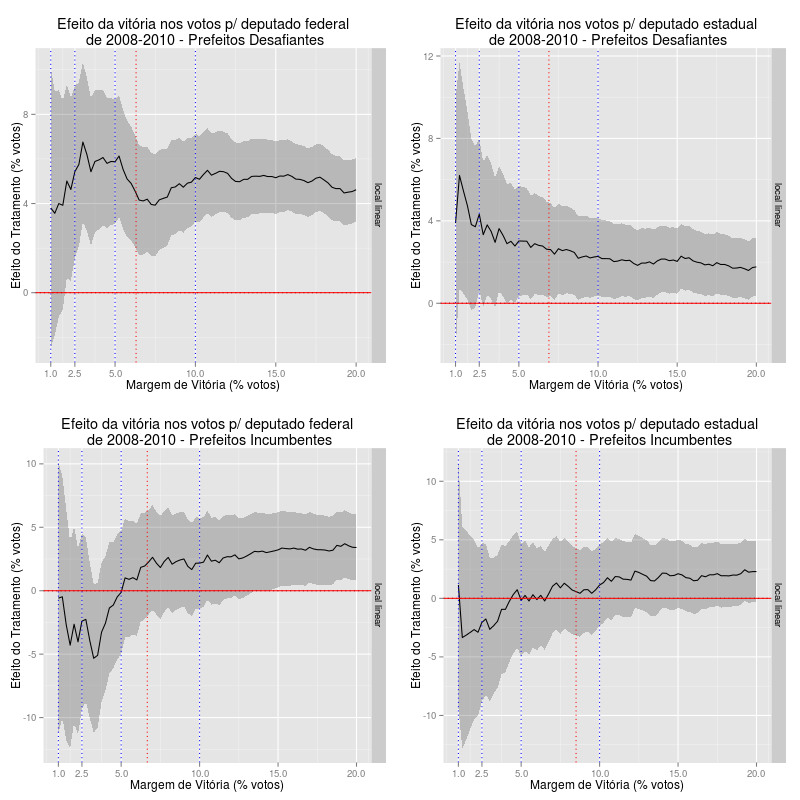
\includegraphics[scale=0.5]{c1g14.png}
	\caption{Efeito do Tratamento no Voto para Deputado Federal e Deputado Estadual nas eleições seguintes por margem de vitória nas eleições para prefeito (2008-2010) por contexto eleitoral local}
	\label{fig:c1g14} 
\end{figure}

Mesmo quando considerado apenas o par de eleições 2008-2010, o efeito não é hetegorêneo para todos as conjunturas políticas e eleitorais locais. Vencer onde o partido já governava tem o mesmo impacto na performance nas eleições seguintes que vencer onde o partido não governava?  Na Figura~\ref{fig:c1g14} os resultados são separados em duas situações: aquelas nas quais o partido buscava reeleição para o Executivo municipal e aquelas em que o partido tentou conquistar uma prefeitura nova. No primeiro caso, portanto, são comparados os casos em que o partido governava o município, mas perdeu a eleição, às situações nas quais o partido governava e saiu vitorioso, obtendo mais um mandato (incumbente derrotado \emph{versus} incumbente vitorioso). No segundo caso são comparadas as situações em que o partido não governava a prefeitura e foi derrotado às situações nas quais o partido venceu as eleições em um município em que não governava (desafiante derrotado \emph{versus} desafiante vitorioso).

O resultado é bastante surpreendente e claro: o efeito de vencer as eleições em um município novo é positivo e maior do que o efeito médio obtido anteriormente, sem a separação entre incumbentes e desafiantes. Para deputado federal, com $\Delta \leq 2,5\%$, o efeito é $\rho=5,4\%$ nos votos válidos; para deputado estadual o efeito é $\rho=4,3\%$. Por outro lado, o efeito não aparece quando são comparados apenas os municípios em que o partido já governava. Diferentemente do que tinhamos até então, a vitória eleitoral em municípios novos e em eleições recentes tem um impacto nítido e significativo no desempenho do partido 

Não há hipóteses na literatura para explicar a diferença entre resultados para desafiantes e incumbentes e este é um problema a ser investigado no futuro. É possível que o fato de ganhar as eleições em um novo município permita ao partido construir uma rede de relações entre apoiadores, financiadores de campanha e outros atores políticos relevantes que até então não existia. Este outro problema é investigado no Capítulo~\ref{cap:mecanismos}.

\subsection{O impacto das eleições para prefeito no Brasil: efeitos heterogêneos eleições para deputado federal e estadual por características municipais}

Os resultados também são bastante heterogêneos por tamanho de município. Novamente, apresento os resultados apenas para o período 2008-2010 e apresento no Anexo os resultados para os demais anos, que, basicamente, são resultados nulos. Curiosamente, a heterogeneidade varia de acordo com o cargo. O efeito da vitória no desempenho para deputado federal ocorre sobretudo nos municípios médios, de 10 a 50 mil habitantes. Nos menores municípios (até 10 mil habitantes), o efeito é bastante mais frágil e menor e só teria significância estatística para as menores margens se fosse adotado um intervalo de confiança e/ou margens de vitória maiores do que 5\%. Para os municípios maiores, não há efeito algum.

Para deputado estadual, porém, o efeito da vitória para prefeito é bastante claro nos menores municípios. Nos municípios médios (10 a 50 mil habitantes), o efeito é menor. O resultado para municípios maiores, porém, é contrário ao que se obteve até agora: os deputados federais de um partido em cidades com mais de 50 mil habitantes têm um desempenho inferior em municípios em que o partido venceu as eleições municipais em relação a municípios em que o partido perdeu.

\begin{figure}[htp]
	\centering
	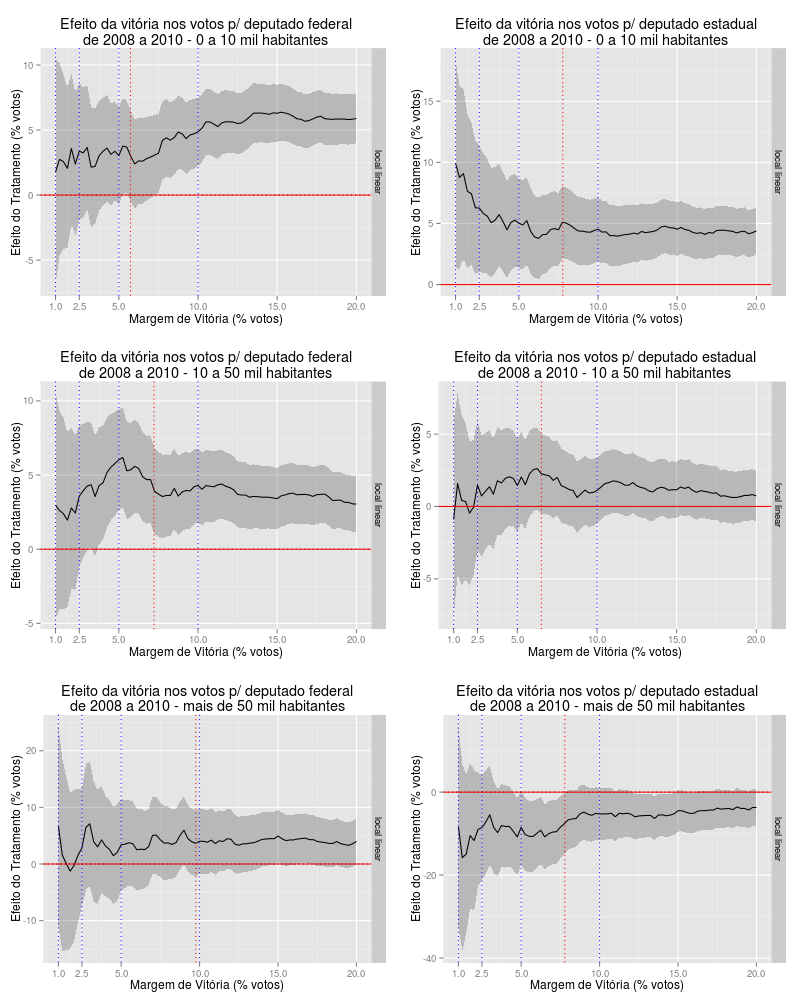
\includegraphics[scale=0.55]{c1g15.png}
	\caption{Efeito do Tratamento no Voto para Deputado Federal e Deputado Estadual nas eleições seguintes por margem de vitória nas eleições para prefeito (2008-2010) por tamanho da população do município}
	\label{fig:c1g15} 
\end{figure}

Portanto, de maneira geral, é nos municípios pequenos e médios que vencer a disputa para prefeito terá efeito relevante no voto para deputado federal e deputado estadual nas eleições seguintes. O resultado não surpreende: em municípios maiores o prefeito disputa com outras liderenças locais a capacidade de articular eleitores e influenciar seu voto. Além disso, nos grandes municípios, há mais votos em disputa e maior acomodação de um grande número de candidatos no sistema proprocional. Em municípios pequenos, a prefeitura é, na maior parte dos casos, o principal acesso dos eleitores ao Estado e a serviços públicos. Ainda que não seja possível testar a hipótese de que prefeitos em cidades menores têm maior ascendência sobre os eleitores, o resultado na Figura~\ref{fig:c1g15} torna esta hipótese mais plausível.

O tamanho do município não é a única característica municipal para a qual há efeitos heterogêneos do tratamanto sobre o desempenho nas eleições para deputado federal e deputado estadual. A Figura~\ref{fig:c1g16} traz os resultados separados por municípios de maior e menor PIB per capita e para os municípios mais e menos dependentes de transferências de receitas. Neste último caso, a medida utilizada é a razão entre as receitas de transferências e as receitas totais. Os grupos foram separados de maneira bastante simples: por quartil na distribuição em cada variável. Para facilitar e sintetizar a visualização dos resultados, apenas o primeiro e o quarto quartil são apresentados e os demais constam no Anexo. A omissão dos quartis centrais não altera a interpretação dos resultado.

\begin{figure}[htp]
	\centering
	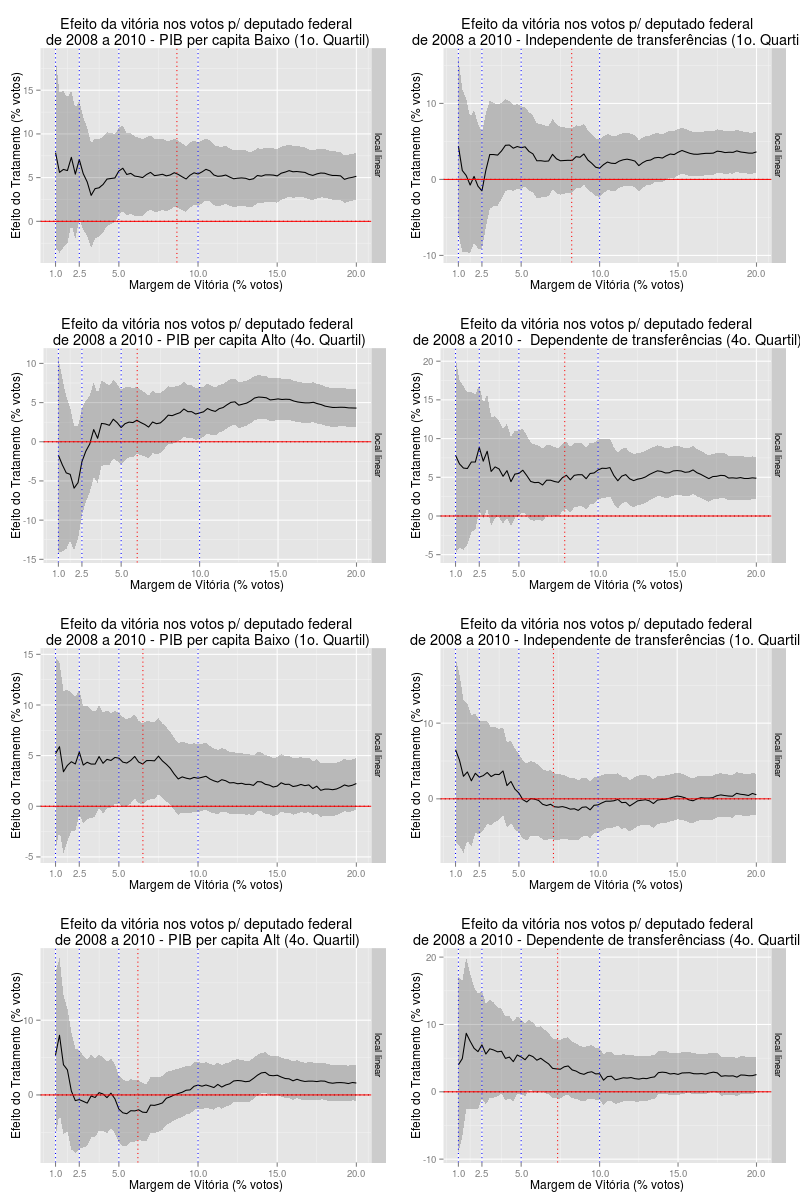
\includegraphics[scale=0.5]{c1g16.png}
	\caption{Efeito do Tratamento no Voto para Deputado Federal e Deputado Estadual nas eleições seguintes por margem de vitórias nas eleições para prefeito (2008-2010) por características econômicas do município (PIB per capita e grau de dependência de transferências de outros níveis de governo)}
	\label{fig:c1g16} 
\end{figure}

Nos municípios com PIB per capita baixo o efeito é maior e mais resistente à redução da margem de vitória do que nos municípios com PIB per capita alto. Municípios com PIB menor são também aqueles cuja população depende em média mais do Estado e, portanto, nos quais as lideranças dos governos municipais têm maior centralidade na cena política e econômica local.

Ambos os resultados apontam, pelo menos hipoteticamente, para um ponto de convergência: o efeito de vencer as eleições para o Executivo municipal será maior em localidades nas quais o prefeito tem papel político e econômico de destaque, ou ainda, enfrenta menos concorrência de liderenças locais e atores econômicos para influenciar a decisão dos eleitores. Dito de outra forma, o impacto do tratamento nas eleições municipais e estaduais é maior onde o prefeito é um cabo eleitoral privilegiado.

Com relação às receitas municipais, o impacto da vitória no município sobre os votos nas eleições proporcionais seguintes chega próximo a 10\% nos municípios mais dependentes de transferências de outros níveis de governo, enquanto nos municípios mais independentes de transferências o impacto não é diferente de zero. Este resultado é particularmente importante para avançarmos ao segundo capítulo. Os municípios nos quais as receitas provenientes dos governos estaduais e governo federal são também aqueles nos quais a ação dos deputados de ambos níveis de governo tem maior impacto político e econômico. Nesses municípios a intermediação dos parlamentares pode trazer retorno eleitoral maior. Como se verá abaixo, pelo menos no caso de deputados federais, os parlamentares não escolhem aleatoriamente prefeituras para onde enviarão recursos inseridos no orçamento mediante emenda parlamentar e privilegiam prefeitos dos próprios partidos. Portanto, além do impacto estar associado à relevância política e econômica do prefeito, também está associado ao impacto que recursos de outros governos produzem no município.

\subsection{O impacto das eleições para prefeito no Brasil: deputados estaduais e federais candidatos à reeleição}

A existência de efeito das eleições para prefeito nos votos para deputado federal e estadual, ainda que restrita às circustâncias apontadas, indica que políticos de um mesmo partido se coordenam entre eleições no Brasil. Isso não significa necessariamente que tal coordenação seja espontânea ou não envolva custos. Não haveria sentido algum em prefeitos apoiarem candidatos pouco competitivos ou que não fossem capazes de, uma vez eleitos, lhes concederem vantagens políticas ou econômicas. Deputados federais e estaduais que buscam a reeleição são, dentre todos os candidatos, alguns dos que tem maiores possibilidades de atrair o apoio de prefeitos para suas candidaturas.

Nessa subseção, apresento os impactos da vitória eleitoral no município separando os candidatos a deputado federal e estadual que buscam um novo mandato dos candidatos desafiantes, que buscam o mandato para aquele cargo pela primeira vez ou que não foram eleitos na disputa anterior.

O procedimento nesta subseção é um pouco diferente do que foi feito até agora. Em vez de construir um subconjunto de observações a partir de uma restrição qualquer (por exemplo, apenas municípios com menos de 10 mil habitantes), separdo $Y_{i}$ em duas partes, $Y_{i,incumbentes}$ e $Y_{i,desafiantes}$, e testo o efeito do tratamento em cada uma delas. Em cada município, um partido pode ter $Y_{i} = Y_{i,incumbentes}+Y_{i,desafiantes}$ votos. Um cuidado importante é não confundir os casos em que os prefeitos são candidatos à releição (que correspondem apenas a uma parcela das observações) com a presente situação, em que a variável dependente é medida de maneira distinta para os deputados à reeleição e para os que não concorrem a um segundo mandato.

\begin{figure}[htp]
	\centering
	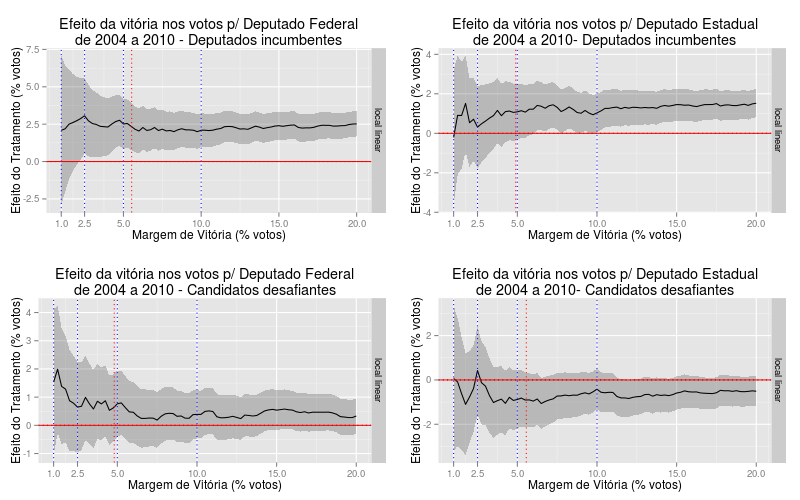
\includegraphics[scale=0.60]{c1g17.png}
	\caption{Efeito do Tratamento no Voto para Deputado Federal e Deputado Estadual nas eleições seguintes por margem de vitórias nas eleições para prefeito (2004-2010), separados por candidatos a deputado incumbentes e desafiantes}
	\label{fig:c1g17} 
\end{figure}

A Figura~\ref{fig:c1g17} apresenta os resultados da separação entre candidatos a deputado incumbentes e candidatos desafiantes, tanto para deputado federal quanto para deputado estadual. O período analisado contempla os pares de eleições 2004-2006 e 2008-2010, para os quais havia dados para acompanhar os candidatos ao longo dos anos. Os resultados para deputado federal são bastante claros: o impacto do partido vencer nas eleições municipais para candidatos incumbentes é posivito. Tomando a margem de vitória $\Delta \leq 2,5\%$, o impacto nos votos dos deputados a federal que disputam por mais um mandato é de 3\%. Por outro lado, não há evidências de que a vitória nas eleições para prefeito tenha algum impacto no desempenho dos candidatos desafiantes. 

Considerando que o conjunto de incumbentes é bastante menor do que o conjunto de desafiantes o resultado acima apresentado é bastante expressivo. Talvez 5\% a mais dos votos em município para um partido não seja um resultado que altere de maneira relevante o resultado eleitoral global. Contudo, 3\% a mais de votos para os candidatos incumbentes em municípios em que o próprio partido governa é uma vantagem expressiva para um conjunto pequeno de candidatos. Mesmo quando os resultados são separados por par de eleição o efeito continua expressivo (omitidos nesta seção e apresentados no Anexo).

Infelizmente não foi possível separar para esta pesquisa os resultados entre candidatos a deputado federal incumbentes e desafiantes para as eleições anteriores a 2004. É possível que a ausência de resultados diferentes de zero para o período, apresentados logo no início desta seção, seja produto da análise indissociada dos dois conjuntos de candidatos, desafiantes e incumbentes. Os resultados anteriores sobre as diferenças entre os períodos devem, portanto, ser repensados à luz destes novos resultados.

No caso de deputados estaduais e para o período todo, 2004 a 2010, não há evidências de que o voto de candidatos incumbentes ou desafiantes sejam afetados pelo resultados das eleições para prefeito anteriores. Os sinais dos coeficientes estimados, entretanto, indicam que deve haver um impacto diferente do tratamento nos votos dos deputados estaduais buscando um novo mandato em comparação com candidatos desafiantes. De fato, os resultados para 2004 (omitidos no texto principal e apresentados no Anexo) apontam que desafiantes tem resultado negativo onde o próprio partido venceu as eleições para prefeito. Algo semelhante ocorre com os desafiantes a deputado federal em 2004, ainda que não haja evidências de que o impacto seja diferente de zero, mesmo que seu sinal seja negativo.

Vamos agora examinar o impacto das eleições para prefeito no Brasil no desempenho de seus candidatos a para senador, governador e presidente.

\section{O impacto das eleições para prefeito no Brasil: eleições para senador, governador e presidente}

Vimos que a vitória nas eleições para prefeito tem impactos no desempenho do partido para deputado federal e estadual nas eleições subsequentes, ainda que este efeito esteja circunscrito às eleições recentes e varie de acordo com o contexto político local e com as características dos municípios. Nesta seção, repito o procedimento de análise para os demais cargos, senador, governador e presidente.

Há uma grande diferença entre as eleições nacionais e estaduais proporcionais e as disputas para o Poder Executivo e para o Senado: o número de cadeiras em competição. Diferentemente do que ocorre com as eleições proporcionais, os partidos não lançam candidatos em todos as disputas e frequentemente participam em coligações ou deixam de concorrer. Assim, a medida da variável $Y_{i}$ é artificialmente igual a zero em municípios em que o partido governa mas, por exemplo, que estão localizados em um estado no qual o partido não participou das eleições para governador ou senador.

Mesmo tendo mais semelhanças entre si do que com as eleições para deputado federal e estadual, as disputas para o Senado e os governos federal e estadual têm diversas peculiaridades. A competição por cadeiras no Senado varia em magnitude a cada ano eleitoral e analisar conjuntamente eleições com uma ou duas cadeiras em disputa pode levar a resultados equivocados. Nas eleições de 1998 e 2002 cada estado da federação elegeu um senador. Em 2002 e 2010, os estados elegeram dois senadores cada.

O número de partidos competitivos em uma eleição é uma restrição que também deve ser observada. Para a análise do impacto do tratamento nos votos para presidente, a restrição do número de vagas em disputa quase que limita a análise a dois partidos, PT e PSDB, com algumas observações provenientes de partidos que disputaram a terceira ou quarta colocação e dos partidos pequenos. Convém lembrar que apenas o PSB (com Anthony Garotinho em 2002) dentre demais partidos participantes das eleições presidenciais é simultaneamente um partido competitivo nas eleições nacionais e municipais. Porém, para simplificar a análise do impacto dos tratamentos no voto para presidente, manterei apenas PSDB e PT na análise.

Por sua vez, nas eleições para governador e senador ocorre algo semelhante, ainda que os partidos que disputam com chances de vitória não sejam necessariamente os mesmos que concorrem na eleição para presidente. Dessa forma, decidi adotar um mecanismo de exclusão dos candidatos a governador e senador. Exlcuí todos os candidatos menos competitivos, que tiveram menos de 15\% dos votos totais no estado quando há apenas uma vaga em disputa e 7,5\% dos votos para as eleições ao Senado quando a competição for por duas vagas.

Uma das alternativas analíticas para este capítulo seria considerar o apoio a candidatos do Executivo de todos os prefeitos envolvidos na coalização. Dessa maneira, $p$ seria definido por qualquer partido aliado. Por exemplo, observaríamos o efeito do PMDB vencer em 2000 na candidatura do PSDB à presidência em 2002, excluiríamos o partido no par de eleições 2004-2006 por não ter apoiado nenhum candidato e incluiríamos o partido novamente em 2008-2010 para examinar o efeito da vitória para prefeito na candidatura presidencial do PT. Entretanto, os resultados, como se verá abaixo, são bastante instáveis e, quando são diferentes de zero, normalmente são negativos. Se quando o próprio partido vence as eleições para prefeito a performance para os cargos do Executivo não melhora, por qual razão a vitória de um aliado na prefeitura deveria importar? Assim, em vez de complexificar a análise neste momento, decidi deixar a avaliação do impacto de um aliado vencer as eleições para prefeito no desempenho eleitoral do partido para trabalhos futuros.

\subsection{O impacto das eleições para prefeito no Brasil: eleições para senador, governador e presidente no período 1996-2010}
 
A Figura~\ref{fig:c1g18} apresenta o impacto da vitória eleitoral nos votos do partido para os três cargos em análise nas eleições seguintes. Os resultados para senador estão separados entre eleições em que há apenas uma (1996 e 2004) ou duas vagas em disputa (2000 e 2004). Em cada um dos gráficos, apresento o resultado pelos três métodos de estimação distintos adotado no capítulo.

\begin{figure}[htp]
	\centering
	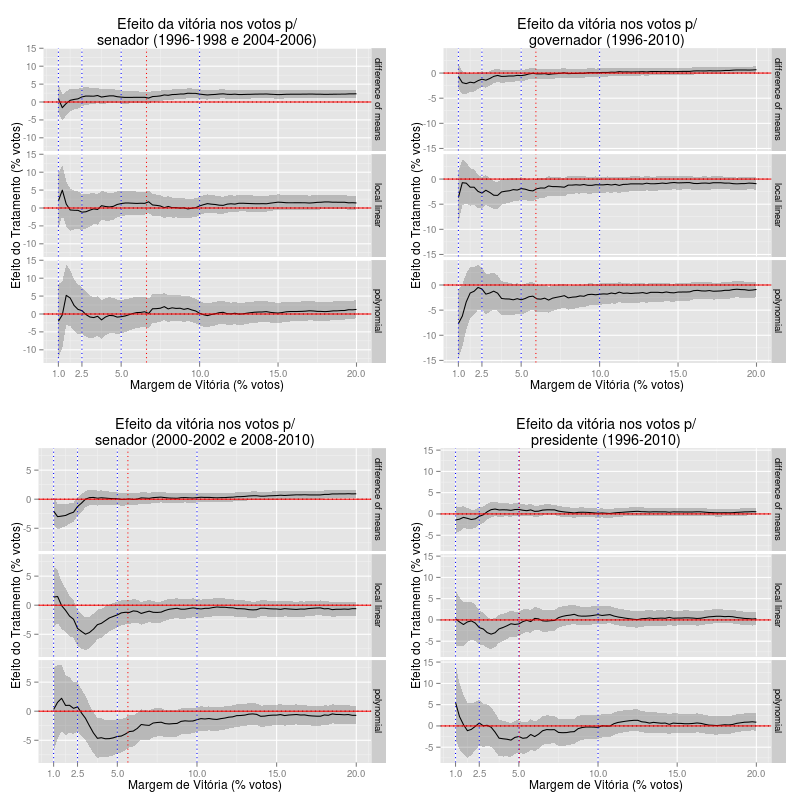
\includegraphics[scale=0.6]{c1g18.png}
	\caption{Efeito do Tratamento no Voto para Senador, Governador e Presidente nas eleições seguintes por margem de vitórias nas eleições para prefeito (1996-2010)}
	\label{fig:c1g18} 
\end{figure}


O exame dos gráficos a Figura~\ref{fig:c1g18} não apenas revela que não há efeitos positivos da vitória para prefeito no desempenho do partido para os demais cargos como também indica que, em alguns casos, o resultado é negativo. Tanto na competição por duas cadeiras no Senado quanto nas disputas para governador ter vencido as eleições anteriores afeta negativamente o desempenho do partido, ainda que sejam evidências um pouco frágeis e mereçam uma análise mais cuidadosa. Diferentemente do que encontrou \citet{Ames1994} para a eleição de 1989, o efeito da vitória municipal nos votos para a presidência é nulo.

Tal como fizemos com a análise do impacto do tratamento sobre os votos para deputado federal e estadual, vamos examinar os potenciais efeitos heterogêneos que contribuem para explicar os resultados da Figura~\ref{fig:c1g18} antes de refletir sobre as implicações teóricas do resultados.

\subsection{O impacto das eleições para prefeito no Brasil: efeitos heretogêneos do tratamento nas eleições para senador}

O efeito negativo da vitória apresentado nas eleições para senador em que há duas vagas em disputa permanece independentemente das características dos municípios ou do contexto político local (se o partido já governava antes de vencer a última eleição para prefeito ou se venceu em um município que não governava). Estes resultados, cuja apresentação no texto principal é irrelevante, são apresentados no Anexo. A separação pelo número de cadeiras no Senado em disputa, consequência da própria regra eleitoral, já contribui para a separação dos resultados por pares de eleição. Se separarmos os pares de eleição 2000-2002 e 2008-2010, os resultados permanecem exatamente inalterados para os dois anos e tampouco há razões para apresentá-los senão no Anexo.

É possível concluir que o efeito negativo para senador é, portanto, constante? Aparentemente não. A Figura~\ref{fig:c1g19} traz o resultado por partido para os dois pares de eleições em que há duas cadeiras em disputa no Senado. Note-se que apenas um partido, o DEM, tem um resultado negativo diferente de zero e correspondente ao padrão geral. O último gráfico da figura apresenta o resultados para todos os partidos exceto o DEM.

\begin{figure}[htp]
	\centering
	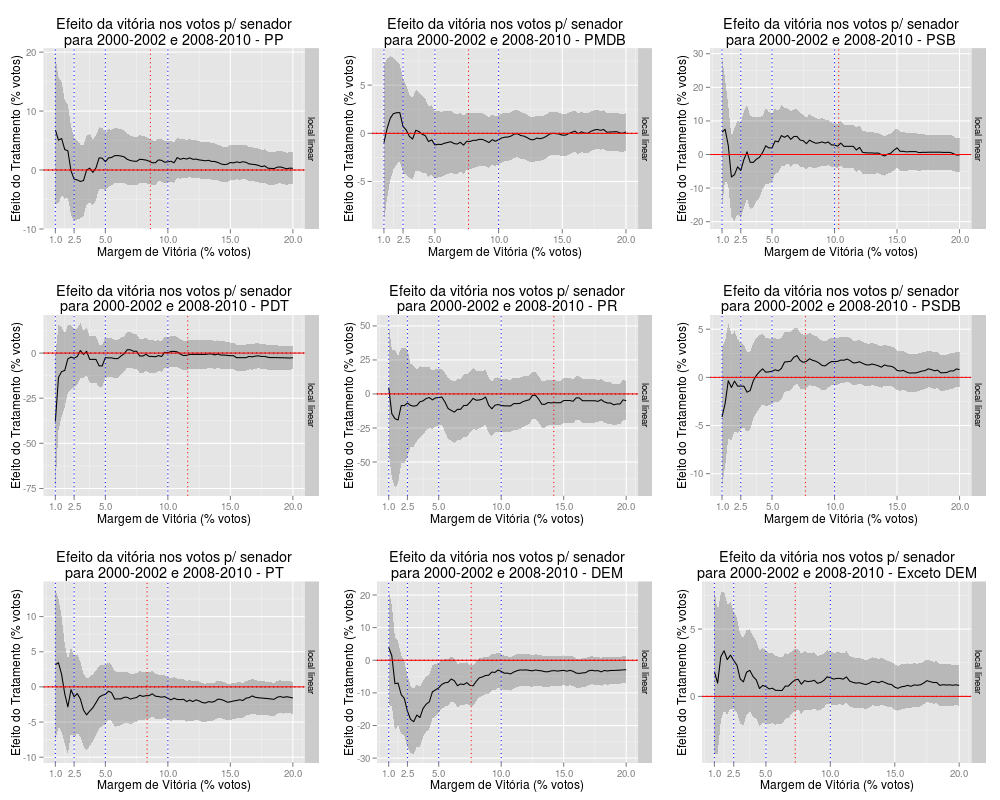
\includegraphics[scale=0.45]{c1g19.png} 
	\caption{Efeito do Tratamento no Voto para Senador nas eleições seguintes por margem de vitórias nas eleições para prefeito (2000-2002 e 2008-2010) por partido}
	\label{fig:c1g19} 
\end{figure}

Claramente, vencer as eleições para prefeito não tem efeito no desempenho do partido nas eleições para senador. O DEM é a exceção e não é a toa. Desde o final do segundo mandato do presidente Fernando Henrique Cardoso, o DEM é um dos maiores derrotados nas urnas. O partido teve a maior bancada de senadores no fim dos anos 1990 e começo dos anos 2000. Hoje, a bancada do partido conta com apenas quatro senadores e as baixas ocorreram tanto em virtude de importantes derrotas eleitorais quanto por migração para outros partidos. De fato, o partido enfrenta uma crise bastante séria e não é estranho esperar que os prefeitos do DEM apoiem eleitoralmente candidatos de outros partidos ao longo dos anos 2000. Em 2011 várias lideranças do DEM migraram para o recém criado PSD. 

Quando consideramos apenas os casos em que há uma cadeira para senador em disputa no estado, o resultado permanece inalterado e não há efeito da vitória nas eleições municipais no desempenho do partido na competição pelo Senado Federal.

A lógica da disputa ao Senado torna a separação entre candidatos incumbentes e desafiantes algo complexo. Diferentemente do que ocorre na competição por cadeiras na Câmara dos Deputados e nas Assembléias Legislativas, o partido terá apenas candidatos desafiantes ou incumbentes nas eleições para uma única vaga, nunca os dois ao mesmo tempo. Em outras eleições, porém, o partido poderá ter só um candidato incumbente, só um desafiante ou os dois. A variedade de arranjos possíveis torna inviável separar a análise do efeito do tratamento entre senadores em busca da continuação do mandato e desafiantes. Podemos concluir que não há efeitos -- positivos ou negavitos -- da vitória nas eleições para prefeito no voto do partido para o Senado, exceto, obviamente, pelo DEM. Vamos agora analisar o impacto da vitória nas eleições para governador. 

\subsection{O impacto das eleições para prefeito no Brasil: efeitos heretogêneos do tratamento nas eleições para governador}

Um aspecto fundamental a se considerar na análise do impacto da vitória municipal na performance do partido para governador é a existência de diferenças entre os candidatos a governador em campanha de reeleição e os candidatos que buscam um primeiro mandato. Governadores são atores importantes localmente e por vezes cruciais para o desenvolvimento político e econômico dos municípios. Ainda que candidatos ao governo do Estado sejam, em geral, políticos com maior ascensão sobre os diretórios locais, governadores são atores bastante poderosos dentro de sua circunscrição. A Figura~\ref{fig:c1g20} traz os resultados para governador separando-os entre candidatos desafiantes ou incumbentes e também por partido desafiante ou incumbente (quando o partido busca mais um mandato sem que o próprio governador esteja concorrendo a mais um mandato). Há evidências frágeis de que governadores (ou seu partido) se beneficiem eleitoralmente da vitória do próprio partido em eleições municipais. Mas o resultado mais relevante é que candidatos desafiantes têm resultado negativo onde o próprio partido ganha. Adotando $\Delta \leq 2,5\%$ como referência, candidatos desafiantes tendem a ter 4,5\% menos votos em municípios nos quais o seu próprio partido venceu as eleições municipais anteriores em relação aos municípios onde seu partido perdeu. 

\begin{figure}[htp]
	\centering
	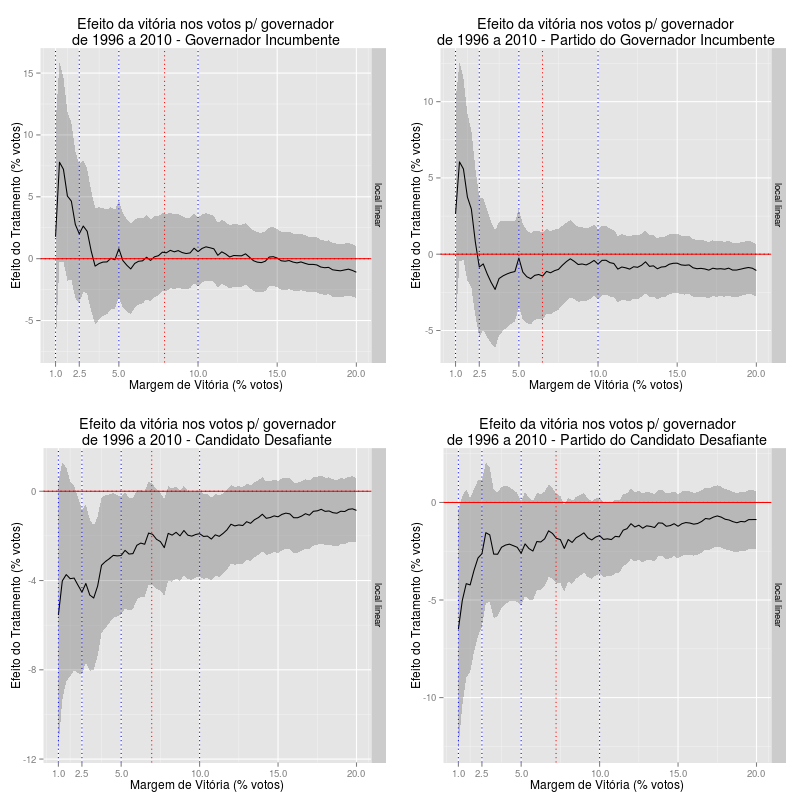
\includegraphics[scale=0.45]{c1g20.png}
	\caption{Efeito do Tratamento no Voto para Governador nas eleições seguintes por margem de vitórias nas eleições para prefeito (1996-2010) para candidatos/partidos incumbentes e desafiantes}
	\label{fig:c1g20} 
\end{figure}

O raciocínio é contra-intuitivo: por qual razão os candidatos desafiantes teriam um desempenho pior nos municípios em que o partido venceu as eleições anteriores? Talvez governadores (ou partidos) em campanha por reeleição concentrem esforços justamente em municípios governados pelos partidos de seus concorrentes. Conquistar prefeitos legendas capazes de trair suas legendes pode ser uma estratégia eleitoralmente mais rentável do que cultivar os prefeitos do próprio partido. Isso explicaria, inclusive, o resultado nulo para candidatos (ou partidos) incumbentes, uma vez que tais candidatos teriam desempenho igualmente positivo onde o partido governa em comparação com locais em que os prefeitos de seus opositores governam. Menos do que uma conclusão, este raciocínio é hipotético e depende de esforços de pesquisa apropriados para investigá-lo com cuidado.

Tal como no caso de senadores, o impacto do tratamento para governador depende menos das características dos municípios ou da conjuntura política municipal do que de outros aspectos da própria competição pelos Executivos estaduais. Alguns resultados apresentados no Anexo apontam que o tratamento é positivo para governadores incumbentes em municípios maiores e que o efeito negativo para desafiantes é mais forte em municípios em que o partido já governa e venceu novamente as eleições. A principal variável que explica a heterogeneidade do efeito do tratamento para governador, porém, continua sendo a condição de incumbente ou desafiante dos candidatos. Dado o escopo desta pesquisa, só é possível oferecer explicações \emph{ad hoc} sobre resultados inesperados.

\subsection{O impacto das eleições para prefeito no Brasil: efeitos heretogêneos do tratamento nas eleições para presidente}

A análise do efeito do tratamento nas eleições presidenciais no período entre 1996 e 2010 é quase equivalente à análise do efeito do tratamento para PT e PSDB na disputa pelo Governo Federal. Convém, portanto, separar o efeito por partido. Além disso, os dois partidos disputam cada uma das quatro eleições em análise em condições variadas, como incumbentes ou como desafiantes, e com casos de reeleição em 1998 e 2006. É de se esperar, portanto, que os efeito sejam heterogêneos para cada eleição e partido. A Figura~\ref{fig:c1g21} apresenta os resultados para os dois partidos para todo o período e também por eleição.

\begin{figure}[htp]
	\centering
	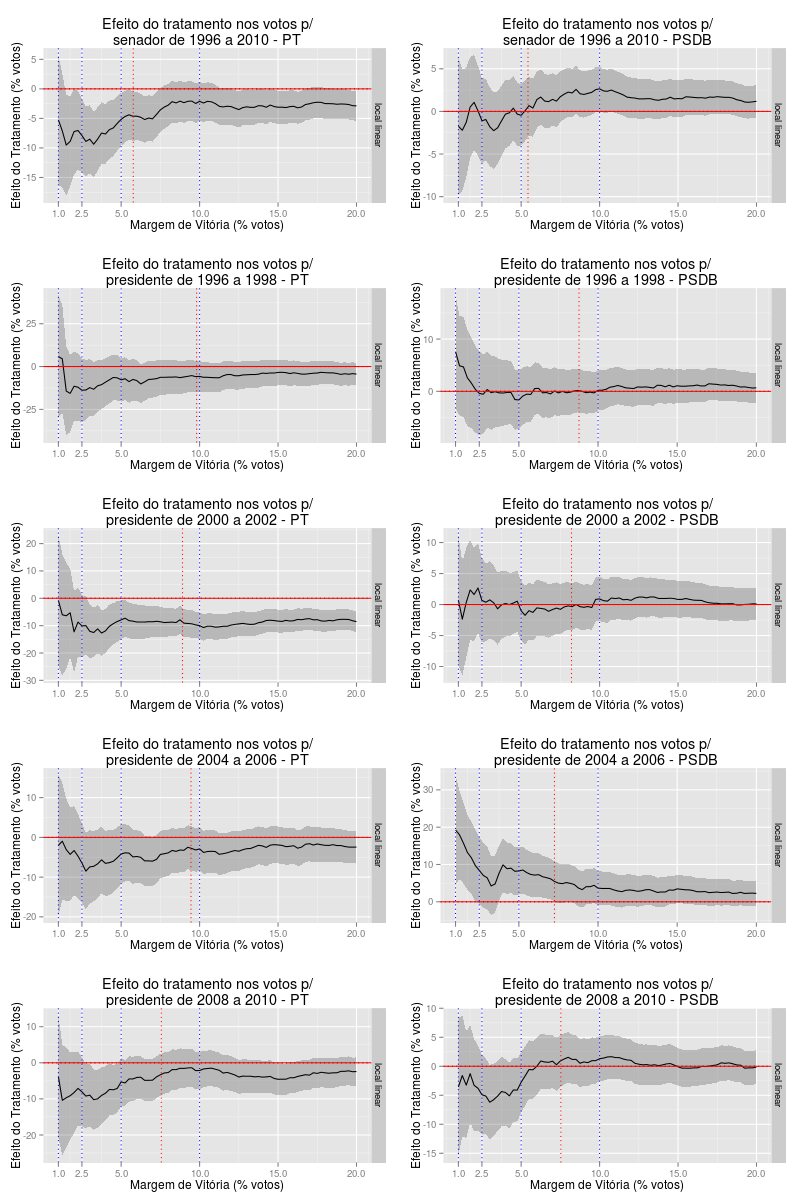
\includegraphics[scale=0.5]{c1g21.png} 
	\caption{Efeito do Tratamento no Voto para Presidente nas eleições seguintes por margem de vitórias nas eleições para prefeito (1996-2010 e por par de eleição) para PT e PSDB}
	\label{fig:c1g21} 
\end{figure}

A separação do resultados por partido aponta para efeitos da vitória eleitoral muito diferentes para PT e PSDB. Claramente, o PT tem um desempenho pior para a presidência nos municípios em que vence as eleições municipais, resultado na contra-mão do que apontou \citet{Ames1994} ao analisar as eleições de 1989. O efeito negativo da vitória é particularmente crítico nas eleições presidenciais de 2002 e 2010 . Adotando a margem de vitória de referência menor ou igual 2,5\%, o efeito do tratamento em 2002 é de -10\% (diferente de zero para nível de significância igual a 90\%) e -8\% (sem, no entanto, ser estatisticamente diferente de zero para esta margem específica). Em 2002 o resultado é bastante compreensível. Tal como no caso dos candidatos a governador desafiantes, o PT era o partido que tentava consquistar a presidência concorrendo com o candidato do PSDB, que governava por dois mandatos consecutivos. Entretanto, em 2010 o PT era o partido no governo. Da mesma forma, o PSDB era o partido desafiante nas duas eleições presidenciais recentes e, contrariamente ao PT, o efeito do tratamento é nulo (2010) ou positivo (2006).

Tampouco é possível argumentar, como se fez na análise do impacto da vitória para prefeito no desempenho para as eleições ao Senado, que o partido com resultados negativos esteja em decadência eleitoral, caso do DEM. Pelo contrário, O PT é o partido mais vitorioso nacionalmente nos últimos anos sob diversos aspectos. A decadência eleitoral do partido não explica os resultados da Figura~\ref{fig:c1g21}.

Os resultados do efeito do tratamento nos votos para senador, presidente e governador demandam investigação mais aprofundada dos mecanismos pelos quais a eleição para prefeito afeta as eleições nacionais e estaduais. Por enquanto, é possível apenas apontar que o efeito da vitória no município é variado, muitas vezes localizados em um partido específico, e em diversas vezes negativo, contrariando os resultados anteriormente obtidos por \citeauthor{Ames1994}.

\section{Conclusões tentativas sobre o impacto da vitória para prefeito nas eleições nacionais/estaduais e questões a serem exploradas no futuro}

O objetivo deste capítulo foi produzir evidências que apontam para a existência de coodernação interna nos partidos brasileiros. A despeito dos incentivos instituiconais contrários, sabemos que há cooperação eleitoral entre candidatos deputado federal e estadual e os prefeitos membros de uma organização partidária. Pelo menos para eleições recentes, os partidos vitoriosos nas eleições municipais têm desempenho melhor nas eleições nacionais e estaduais para o Legislativo na localidade do que os partidos derrotados e que este efeito pode ocorrer apenas se houver cooperação entre políticos de um mesmo partido.

Os resultados apresentados no capítulo, contudo, são bastante instáveis. Há várias situações para as quais o efeito da vitória nas candidaturas do partido à Camara dos Deputados e Assembléias Legislativas inexiste. O destaque a resultados positivos dado em alguns momentos ao longo da análise reside na crença de que a estratégia de investigação favorece a obtenção de resultados nulos e, portanto, a obtenção de algum resultado -- positivo ou negativo -- deve ser tomada como uma evidência empírica importante. Em mais de um momento, o impacto do tratamento nos votos nas eleições legislativas seguintes era positivo e, assim, parece adequado assumir a existência de efeito como a principal conclusão deste primeiro capítulo.

Os efeitos do tratamento no voto do partido para os demais cargos -- senador, governador e presidente -- observados no capítulo, por outro lado, não permitem qualquer conclusão. Servem unicamente para destacar as diferenças de senadores com os demais legisladores e apontar que ainda há que se aprimorar as formas de investigar se os destinos eleitorais dos candidatos ao Executivo em diferentes níveis de governo está entreleçado.

O esforço investigativo empreendido nesta primeira etapa da tese tem alguns caminhos a seguir no futuro. O primeiro deles é ampliar a série de dados com os resultados eleitorais de 2014. Se, como apontei anteriormente, o amadurecimento do sistema partidário brasileiro é uma das possíveis causas para a mudança dos padrões de relação entre prefeitos e deputados federais e estaduais variar ao longo do tempo, a inclusão de disputas futuras será de grande proveito para a análise.

Além disso, apontei em alguns momentos para o efeito distorsivo que a migração de prefeitos pode provocar na análise. Contemplar a migração de prefeitos deve ser um importante objetivo do prosseguimento desta pesquisa.

Finalmente, a narrativa sustentada no capítulo sobre a existência de coordenação entre membros de um partido em diferentes níveis de governo pode ser complementada com outra formas de investigação. Em particular, seria bastante interessante acompanhar como prefeitos se envolvem nas candidaturas de deputados federais e estaduais e como as liderenças partidárias decidem (ou não decidem) distribuir o apoio político dos prefeitos entre os concorrentes de sua legenda. Infelizmente o momento de elaboração da tese não coincidiu com as eleições nacionais e estaduais, momento no qual tais problemas podem ser investigados.

A maneira encontrada para prosseguir com o tema foi investigar questões correlatas sobre coordenação dentro dos partidos politicos brasileiros aproveitando as virtudes do desenho de regressão descontínua. No próximo capítulo procuro investigar a conexão entre deputados federais e prefeitos tem reflexos também na arena legislativa.